\chapter{Алгоритм на основе восходящего анализа}

Традиционно, алгоритмы, применяемые для анализа языков программирования как раз умеют строить дерево разбора --- то, что нам надо.
Только нам бы лес.
Вот и посмотрим, как это можно сделать.

Сперва поговорим про классический синтаксический анализ, потом про его адаптацию к анализу графов.

\section{Восходящий синтаксический анализ}

LR(k) --- алгоритм восходящего синтаксического анализа. 
Идея заключается в следующем: входная последовательность символов считывается слева направо с попутным добавлением в стек и выполнением сворачивания --- замены последовательности терминалов и нетерминалов, лежащих наверху стека, на нетерминал, если существует соответствующее правило в исходной грамматике.

\begin{definition}
Слот (item) --- правило грамматики, в правой части которого имеется точка, отделяющая уже разобранную часть правила (слева от точки) от того, что еще предстоит распознать (справа от точки).
\end{definition}

\begin{definition}
LR-автомат --- автомат с магазинной памятью, состояния которого задаются ``слотами'', также он имеет следующий набор инструкций: \\
1. shift p --- прочитать следующий символ входной последовательности, положив его в стек, и перейти в состояние p \\
2. reduce k --- применить k-ое правило грамматики, правая часть которого уже лежит на стеке: снимаем правую часть и кладём левую часть
\end{definition}

\begin{definition}
Предпросмотр --- метод, применяемый в синтаксическом анализе. Заключается в следующем: устанавливается максимальное количество входящих символов, которое может быть использовано анализатором для решения того, какое правило использовать (в случае восходящего анализа: к какому правилу нужно свернуться).
\end{definition}

\begin{definition}
Управляющая таблица --- таблица, которая для всех состояний LR-автомата содержит: инструкции для выполнения, если на вершине стека --- терминал (при этом в случае LR(k) в каждой ячейке может находиться не более одной инструкции), номер состояния, в которое нужно перейти, если на вершине стека --- нетерминал.
\end{definition}

Когда в текущем состоянии '.' стоит в конце, мы можем выполнить reduce-инструкцию и перейти в новое состояние. Однако при этом могут возникать следующие конфликты:
\begin{itemize}
\item shift-reduce --- ситуация, когда не понятно, читать ли следующий символ или выполнить reduce. Например, если правая часть одного из правил является префиксом правой части другого правила: $N \rightarrow w, M \rightarrow ww'$.
\item reduce-reduce --- ситуация, когда не понятно, к какому правилу нужно применить reduce. Например, если есть два правила с одинаковыми правыми частями: $N \rightarrow w, M \rightarrow w$.
\end{itemize}

Возьмем следующую грамматику:
\begin{align*}
0) S & \rightarrow a S b S \\
1) S & \rightarrow \varepsilon
\end{align*}

Расширим вышеупомянутую грамматику, добавив новый стартовый нетерминал S', и далее будем работать с этой расширенной грамматикой:
\begin{align*}
0) & S \rightarrow a S b S \\
1) & S \rightarrow \varepsilon \\
2) & S' \rightarrow S \$
\end{align*}

\begin{definition}
Замыкание --- обобщение понятия ``item'', заключающееся в добавлении для каждого item'а вида $N \rightarrow \alpha.M\beta$ item'ов вида $M \rightarrow .\gamma$
\end{definition}

\begin{definition}
Ядро --- исходный item, до применения к нему замыкания.
\end{definition}

\begin{example}
Пример ядра и замыкания. 

Возьмем правило 2 нашей грамматики, предположим, что мы только начинаем разбирать данное правило.

Ядром в таком случае является item исходного правила: $S' \rightarrow .S \$$

При замыкании добавятся ещё два item'a с правилами по выводу нетерминала 'S', поэтому получаем три item'a: $S' \rightarrow .S\$$, $S \rightarrow .aSbS$ и $S \rightarrow .\varepsilon$
\end{example}

\begin{example}
Пример построения LR-автомата для нашей грамматики с применением замыкания.
\begin{enumerate}
\item Добавляем стартовое состояние: item правила 0 и его замыкание (вместо item'a $S \rightarrow .\varepsilon$ будем писать $S \rightarrow .$). \\ \\
\tikzset{every picture/.style={line width=0.75pt}}
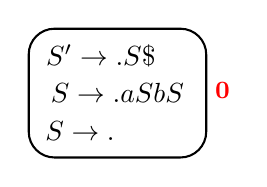
\begin{tikzpicture}[x=0.75pt,y=0.75pt,yscale=-1,xscale=1]
%Rounded Rect
\draw   (139.33,32.07) .. controls (139.33,25.22) and (144.89,19.67) .. (151.74,19.67) -- (212.44,19.67) .. controls (219.29,19.67) and (224.85,25.22) .. (224.85,32.07) -- (224.85,69.3) .. controls (224.85,76.15) and (219.29,81.71) .. (212.44,81.71) -- (151.74,81.71) .. controls (144.89,81.71) and (139.33,76.15) .. (139.33,69.3) -- cycle ;
\draw (174.09,32.69) node  [align=left] {$S' \rightarrow .S\$$};
\draw (182.09,50.69) node  [align=left] {$S \rightarrow .aSbS$};
\draw (164,69) node  [align=left] {$S \rightarrow .$};
\draw (232.67,49.33) node  [align=left] {\textbf{{\small \textcolor{red}{0}}}};
\end{tikzpicture}

\item По 'S' добавляем переход из стартового состояния в новое состояние 1. \\ \\
\tikzset{every picture/.style={line width=0.75pt}}
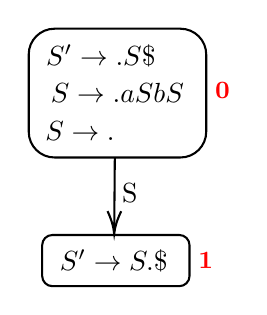
\begin{tikzpicture}[x=0.75pt,y=0.75pt,yscale=-1,xscale=1]
%Rounded Rect
\draw   (139.33,32.07) .. controls (139.33,25.22) and (144.89,19.67) .. (151.74,19.67) -- (212.44,19.67) .. controls (219.29,19.67) and (224.85,25.22) .. (224.85,32.07) -- (224.85,69.3) .. controls (224.85,76.15) and (219.29,81.71) .. (212.44,81.71) -- (151.74,81.71) .. controls (144.89,81.71) and (139.33,76.15) .. (139.33,69.3) -- cycle ;
%Rounded Rect
\draw   (145.81,123.98) .. controls (145.81,121.26) and (148.02,119.05) .. (150.74,119.05) -- (211.87,119.05) .. controls (214.6,119.05) and (216.81,121.26) .. (216.81,123.98) -- (216.81,138.78) .. controls (216.81,141.51) and (214.6,143.72) .. (211.87,143.72) -- (150.74,143.72) .. controls (148.02,143.72) and (145.81,141.51) .. (145.81,138.78) -- cycle ;
%Straight Lines 
\draw    (180.81,81.92) -- (180.53,116.51) ;
\draw [shift={(180.51,118.51)}, rotate = 270.47] [color={rgb, 255:red, 0; green, 0; blue, 0 }  ][line width=0.75]    (10.93,-3.29) .. controls (6.95,-1.4) and (3.31,-0.3) .. (0,0) .. controls (3.31,0.3) and (6.95,1.4) .. (10.93,3.29)   ;
\draw (174.09,32.69) node  [align=left] {$S' \rightarrow .S\$$};
\draw (182.09,50.69) node  [align=left] {$S \rightarrow .aSbS$};
\draw (164,69) node  [align=left] {$S \rightarrow .$};
\draw (180.33,131.67) node  [align=left] {$S' \rightarrow S.\$$};
\draw (188,99) node  [align=left] {S};
\draw (232.67,49.33) node  [align=left] {\textbf{{\small \textcolor{red}{0}}}};
\draw (224.67,131.33) node  [align=left] {\textbf{{\small \textcolor{red}{1}}}};
\end{tikzpicture}

\item По '\$' добавляем переход из состояния 1 в новое состояние 2. \\ \\
\tikzset{every picture/.style={line width=0.75pt}}
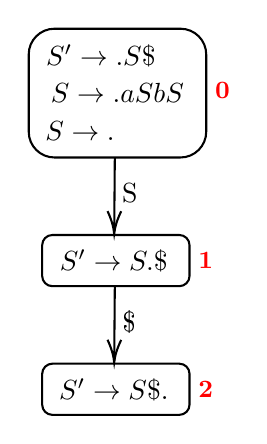
\begin{tikzpicture}[x=0.75pt,y=0.75pt,yscale=-1,xscale=1]
%Rounded Rect
\draw   (139.33,32.07) .. controls (139.33,25.22) and (144.89,19.67) .. (151.74,19.67) -- (212.44,19.67) .. controls (219.29,19.67) and (224.85,25.22) .. (224.85,32.07) -- (224.85,69.3) .. controls (224.85,76.15) and (219.29,81.71) .. (212.44,81.71) -- (151.74,81.71) .. controls (144.89,81.71) and (139.33,76.15) .. (139.33,69.3) -- cycle ;
%Rounded Rect
\draw   (145.81,123.98) .. controls (145.81,121.26) and (148.02,119.05) .. (150.74,119.05) -- (211.87,119.05) .. controls (214.6,119.05) and (216.81,121.26) .. (216.81,123.98) -- (216.81,138.78) .. controls (216.81,141.51) and (214.6,143.72) .. (211.87,143.72) -- (150.74,143.72) .. controls (148.02,143.72) and (145.81,141.51) .. (145.81,138.78) -- cycle ;
%Rounded Rect
\draw   (145.81,185.98) .. controls (145.81,183.26) and (148.02,181.05) .. (150.74,181.05) -- (211.87,181.05) .. controls (214.6,181.05) and (216.81,183.26) .. (216.81,185.98) -- (216.81,200.78) .. controls (216.81,203.51) and (214.6,205.72) .. (211.87,205.72) -- (150.74,205.72) .. controls (148.02,205.72) and (145.81,203.51) .. (145.81,200.78) -- cycle ;
%Straight Lines 
\draw    (180.81,81.92) -- (180.53,116.51) ;
\draw [shift={(180.51,118.51)}, rotate = 270.47] [color={rgb, 255:red, 0; green, 0; blue, 0 }  ][line width=0.75]    (10.93,-3.29) .. controls (6.95,-1.4) and (3.31,-0.3) .. (0,0) .. controls (3.31,0.3) and (6.95,1.4) .. (10.93,3.29)   ;
%Straight Lines 
\draw    (180.81,143.92) -- (180.53,178.51) ;
\draw [shift={(180.51,180.51)}, rotate = 270.47] [color={rgb, 255:red, 0; green, 0; blue, 0 }  ][line width=0.75]    (10.93,-3.29) .. controls (6.95,-1.4) and (3.31,-0.3) .. (0,0) .. controls (3.31,0.3) and (6.95,1.4) .. (10.93,3.29)   ;
\draw (174.09,32.69) node  [align=left] {$S' \rightarrow .S\$$};
\draw (182.09,50.69) node  [align=left] {$S \rightarrow .aSbS$};
\draw (164,69) node  [align=left] {$S \rightarrow .$};
\draw (180.33,131.67) node  [align=left] {$S' \rightarrow S.\$$};
\draw (180.33,193.67) node  [align=left] {$S' \rightarrow S\$.$};
\draw (188,99) node  [align=left] {S};
\draw (188,161) node  [align=left] {\$};
\draw (232.67,49.33) node  [align=left] {\textbf{{\small \textcolor{red}{0}}}};
\draw (224.67,131.33) node  [align=left] {\textbf{{\small \textcolor{red}{1}}}};
\draw (224.67,193.33) node  [align=left] {\textbf{{\small \textcolor{red}{2}}}};
\end{tikzpicture}

\item По 'a' добавляем переход из стартового состояния в новое состояние 3 и делаем его замыкание. Также добавляем переход по 'a' из этого состояния в себя же. \\ \\
\tikzset{every picture/.style={line width=0.75pt}}
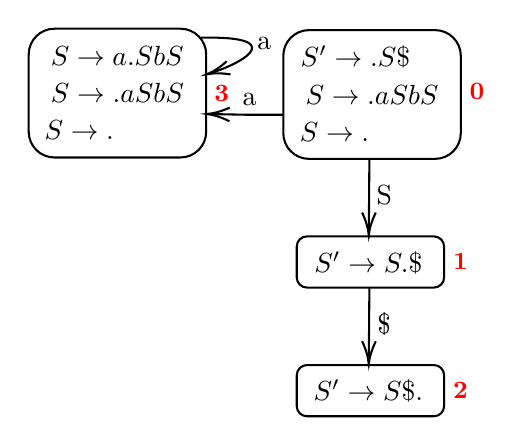
\begin{tikzpicture}[x=0.75pt,y=0.75pt,yscale=-1,xscale=1]
%Rounded Rect
\draw   (139.33,32.07) .. controls (139.33,25.22) and (144.89,19.67) .. (151.74,19.67) -- (212.44,19.67) .. controls (219.29,19.67) and (224.85,25.22) .. (224.85,32.07) -- (224.85,69.3) .. controls (224.85,76.15) and (219.29,81.71) .. (212.44,81.71) -- (151.74,81.71) .. controls (144.89,81.71) and (139.33,76.15) .. (139.33,69.3) -- cycle ;
%Rounded Rect
\draw   (145.81,123.98) .. controls (145.81,121.26) and (148.02,119.05) .. (150.74,119.05) -- (211.87,119.05) .. controls (214.6,119.05) and (216.81,121.26) .. (216.81,123.98) -- (216.81,138.78) .. controls (216.81,141.51) and (214.6,143.72) .. (211.87,143.72) -- (150.74,143.72) .. controls (148.02,143.72) and (145.81,141.51) .. (145.81,138.78) -- cycle ;
%Rounded Rect
\draw   (145.81,185.98) .. controls (145.81,183.26) and (148.02,181.05) .. (150.74,181.05) -- (211.87,181.05) .. controls (214.6,181.05) and (216.81,183.26) .. (216.81,185.98) -- (216.81,200.78) .. controls (216.81,203.51) and (214.6,205.72) .. (211.87,205.72) -- (150.74,205.72) .. controls (148.02,205.72) and (145.81,203.51) .. (145.81,200.78) -- cycle ;
%Rounded Rect 
\draw   (16.67,31.41) .. controls (16.67,24.56) and (22.22,19) .. (29.07,19) -- (89.77,19) .. controls (96.62,19) and (102.18,24.56) .. (102.18,31.41) -- (102.18,68.63) .. controls (102.18,75.48) and (96.62,81.04) .. (89.77,81.04) -- (29.07,81.04) .. controls (22.22,81.04) and (16.67,75.48) .. (16.67,68.63) -- cycle ;
%Straight Lines 
\draw    (180.81,81.92) -- (180.53,116.51) ;
\draw [shift={(180.51,118.51)}, rotate = 270.47] [color={rgb, 255:red, 0; green, 0; blue, 0 }  ][line width=0.75]    (10.93,-3.29) .. controls (6.95,-1.4) and (3.31,-0.3) .. (0,0) .. controls (3.31,0.3) and (6.95,1.4) .. (10.93,3.29)   ;
%Straight Lines 
\draw    (180.81,143.92) -- (180.53,178.51) ;
\draw [shift={(180.51,180.51)}, rotate = 270.47] [color={rgb, 255:red, 0; green, 0; blue, 0 }  ][line width=0.75]    (10.93,-3.29) .. controls (6.95,-1.4) and (3.31,-0.3) .. (0,0) .. controls (3.31,0.3) and (6.95,1.4) .. (10.93,3.29)   ;
%Straight Lines
\draw    (139.5,60.47) -- (122.5,60.47) -- (104.51,60.12) ;
\draw [shift={(102.51,60.09)}, rotate = 361.09000000000003] [color={rgb, 255:red, 0; green, 0; blue, 0 }  ][line width=0.75]    (10.93,-3.29) .. controls (6.95,-1.4) and (3.31,-0.3) .. (0,0) .. controls (3.31,0.3) and (6.95,1.4) .. (10.93,3.29)   ;
%Curve Lines
\draw    (99.51,23.34) .. controls (140.25,22.37) and (122.65,34.57) .. (104.22,40.43) ;
\draw [shift={(102.51,40.96)}, rotate = 343.53999999999996] [color={rgb, 255:red, 0; green, 0; blue, 0 }  ][line width=0.75]    (10.93,-3.29) .. controls (6.95,-1.4) and (3.31,-0.3) .. (0,0) .. controls (3.31,0.3) and (6.95,1.4) .. (10.93,3.29)   ;
\draw (174.09,32.69) node  [align=left] {$S' \rightarrow .S\$$};
\draw (182.09,50.69) node  [align=left] {$S \rightarrow .aSbS$};
\draw (164,69) node  [align=left] {$S \rightarrow .$};
\draw (180.33,131.67) node  [align=left] {$S' \rightarrow S.\$$};
\draw (180.33,193.67) node  [align=left] {$S' \rightarrow S\$.$};
\draw (59.33,32.33) node  [align=left] {$S \rightarrow a.SbS$};
\draw (59.42,50.02) node  [align=left] {$S \rightarrow .aSbS$};
\draw (41,68) node  [align=left] {$S \rightarrow .$};
\draw (188,99) node  [align=left] {S};
\draw (188,161) node  [align=left] {\$};
\draw (123,53) node  [align=left] {a};
\draw (130,26) node  [align=left] {a};
\draw (232.67,49.33) node  [align=left] {\textbf{{\small \textcolor{red}{0}}}};
\draw (224.67,131.33) node  [align=left] {\textbf{{\small \textcolor{red}{1}}}};
\draw (224.67,193.33) node  [align=left] {\textbf{{\small \textcolor{red}{2}}}};
\draw (109.67,50.33) node  [align=left] {\textbf{{\small \textcolor{red}{3}}}};
\end{tikzpicture}

\item По 'S' добавляем переход из состояния 3 в новое состояние 4. \\ \\
\tikzset{every picture/.style={line width=0.75pt}}
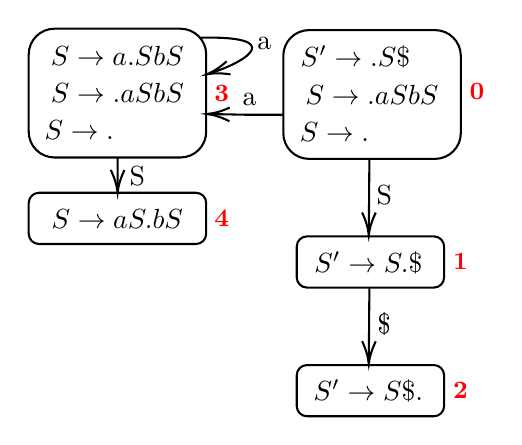
\begin{tikzpicture}[x=0.75pt,y=0.75pt,yscale=-1,xscale=1]
%Rounded Rect
\draw   (139.33,32.07) .. controls (139.33,25.22) and (144.89,19.67) .. (151.74,19.67) -- (212.44,19.67) .. controls (219.29,19.67) and (224.85,25.22) .. (224.85,32.07) -- (224.85,69.3) .. controls (224.85,76.15) and (219.29,81.71) .. (212.44,81.71) -- (151.74,81.71) .. controls (144.89,81.71) and (139.33,76.15) .. (139.33,69.3) -- cycle ;
%Rounded Rect
\draw   (145.81,123.98) .. controls (145.81,121.26) and (148.02,119.05) .. (150.74,119.05) -- (211.87,119.05) .. controls (214.6,119.05) and (216.81,121.26) .. (216.81,123.98) -- (216.81,138.78) .. controls (216.81,141.51) and (214.6,143.72) .. (211.87,143.72) -- (150.74,143.72) .. controls (148.02,143.72) and (145.81,141.51) .. (145.81,138.78) -- cycle ;
%Rounded Rect
\draw   (145.81,185.98) .. controls (145.81,183.26) and (148.02,181.05) .. (150.74,181.05) -- (211.87,181.05) .. controls (214.6,181.05) and (216.81,183.26) .. (216.81,185.98) -- (216.81,200.78) .. controls (216.81,203.51) and (214.6,205.72) .. (211.87,205.72) -- (150.74,205.72) .. controls (148.02,205.72) and (145.81,203.51) .. (145.81,200.78) -- cycle ;
%Rounded Rect 
\draw   (16.67,31.41) .. controls (16.67,24.56) and (22.22,19) .. (29.07,19) -- (89.77,19) .. controls (96.62,19) and (102.18,24.56) .. (102.18,31.41) -- (102.18,68.63) .. controls (102.18,75.48) and (96.62,81.04) .. (89.77,81.04) -- (29.07,81.04) .. controls (22.22,81.04) and (16.67,75.48) .. (16.67,68.63) -- cycle ;
%Rounded Rect
\draw   (16.67,102.98) .. controls (16.67,100.26) and (18.88,98.05) .. (21.6,98.05) -- (97.25,98.05) .. controls (99.97,98.05) and (102.18,100.26) .. (102.18,102.98) -- (102.18,117.78) .. controls (102.18,120.51) and (99.97,122.72) .. (97.25,122.72) -- (21.6,122.72) .. controls (18.88,122.72) and (16.67,120.51) .. (16.67,117.78) -- cycle ;
%Straight Lines 
\draw    (180.81,81.92) -- (180.53,116.51) ;
\draw [shift={(180.51,118.51)}, rotate = 270.47] [color={rgb, 255:red, 0; green, 0; blue, 0 }  ][line width=0.75]    (10.93,-3.29) .. controls (6.95,-1.4) and (3.31,-0.3) .. (0,0) .. controls (3.31,0.3) and (6.95,1.4) .. (10.93,3.29)   ;
%Straight Lines 
\draw    (180.81,143.92) -- (180.53,178.51) ;
\draw [shift={(180.51,180.51)}, rotate = 270.47] [color={rgb, 255:red, 0; green, 0; blue, 0 }  ][line width=0.75]    (10.93,-3.29) .. controls (6.95,-1.4) and (3.31,-0.3) .. (0,0) .. controls (3.31,0.3) and (6.95,1.4) .. (10.93,3.29)   ;
%Straight Lines
\draw    (139.5,60.47) -- (122.5,60.47) -- (104.51,60.12) ;
\draw [shift={(102.51,60.09)}, rotate = 361.09000000000003] [color={rgb, 255:red, 0; green, 0; blue, 0 }  ][line width=0.75]    (10.93,-3.29) .. controls (6.95,-1.4) and (3.31,-0.3) .. (0,0) .. controls (3.31,0.3) and (6.95,1.4) .. (10.93,3.29)   ;
%Curve Lines
\draw    (99.51,23.34) .. controls (140.25,22.37) and (122.65,34.57) .. (104.22,40.43) ;
\draw [shift={(102.51,40.96)}, rotate = 343.53999999999996] [color={rgb, 255:red, 0; green, 0; blue, 0 }  ][line width=0.75]    (10.93,-3.29) .. controls (6.95,-1.4) and (3.31,-0.3) .. (0,0) .. controls (3.31,0.3) and (6.95,1.4) .. (10.93,3.29)   ;
%Straight Lines
\draw    (59.51,81.05) -- (59.5,90) -- (59.5,96) ;
\draw [shift={(59.5,98)}, rotate = 270.03] [color={rgb, 255:red, 0; green, 0; blue, 0 }  ][line width=0.75]    (10.93,-3.29) .. controls (6.95,-1.4) and (3.31,-0.3) .. (0,0) .. controls (3.31,0.3) and (6.95,1.4) .. (10.93,3.29)   ;
\draw (174.09,32.69) node  [align=left] {$S' \rightarrow .S\$$};
\draw (182.09,50.69) node  [align=left] {$S \rightarrow .aSbS$};
\draw (164,69) node  [align=left] {$S \rightarrow .$};
\draw (180.33,131.67) node  [align=left] {$S' \rightarrow S.\$$};
\draw (180.33,193.67) node  [align=left] {$S' \rightarrow S\$.$};
\draw (59.33,32.33) node  [align=left] {$S \rightarrow a.SbS$};
\draw (59.42,50.02) node  [align=left] {$S \rightarrow .aSbS$};
\draw (41,68) node  [align=left] {$S \rightarrow .$};
\draw (59.33,110.67) node  [align=left] {$S \rightarrow aS.bS$};
\draw (188,99) node  [align=left] {S};
\draw (188,161) node  [align=left] {\$};
\draw (123,53) node  [align=left] {a};
\draw (130,26) node  [align=left] {a};
\draw (69,90) node  [align=left] {S};
\draw (232.67,49.33) node  [align=left] {\textbf{{\small \textcolor{red}{0}}}};
\draw (224.67,131.33) node  [align=left] {\textbf{{\small \textcolor{red}{1}}}};
\draw (224.67,193.33) node  [align=left] {\textbf{{\small \textcolor{red}{2}}}};
\draw (109.67,50.33) node  [align=left] {\textbf{{\small \textcolor{red}{3}}}};
\draw (109.67,110.33) node  [align=left] {\textbf{{\small \textcolor{red}{4}}}};
\end{tikzpicture}

\item По 'b' добавляем переход из состояния 4 в новое состояние 5 и делаем его замыкание. Также добавляем переход по 'a' из этого состояния в состояние 3. \\ \\
\tikzset{every picture/.style={line width=0.75pt}}
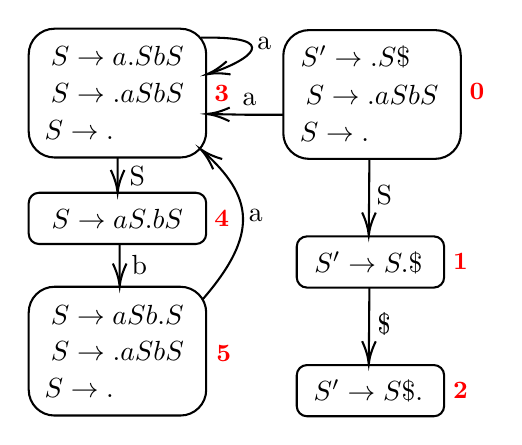
\begin{tikzpicture}[x=0.75pt,y=0.75pt,yscale=-1,xscale=1]
%Rounded Rect
\draw   (139.33,32.07) .. controls (139.33,25.22) and (144.89,19.67) .. (151.74,19.67) -- (212.44,19.67) .. controls (219.29,19.67) and (224.85,25.22) .. (224.85,32.07) -- (224.85,69.3) .. controls (224.85,76.15) and (219.29,81.71) .. (212.44,81.71) -- (151.74,81.71) .. controls (144.89,81.71) and (139.33,76.15) .. (139.33,69.3) -- cycle ;
%Rounded Rect
\draw   (145.81,123.98) .. controls (145.81,121.26) and (148.02,119.05) .. (150.74,119.05) -- (211.87,119.05) .. controls (214.6,119.05) and (216.81,121.26) .. (216.81,123.98) -- (216.81,138.78) .. controls (216.81,141.51) and (214.6,143.72) .. (211.87,143.72) -- (150.74,143.72) .. controls (148.02,143.72) and (145.81,141.51) .. (145.81,138.78) -- cycle ;
%Rounded Rect
\draw   (145.81,185.98) .. controls (145.81,183.26) and (148.02,181.05) .. (150.74,181.05) -- (211.87,181.05) .. controls (214.6,181.05) and (216.81,183.26) .. (216.81,185.98) -- (216.81,200.78) .. controls (216.81,203.51) and (214.6,205.72) .. (211.87,205.72) -- (150.74,205.72) .. controls (148.02,205.72) and (145.81,203.51) .. (145.81,200.78) -- cycle ;
%Rounded Rect 
\draw   (16.67,31.41) .. controls (16.67,24.56) and (22.22,19) .. (29.07,19) -- (89.77,19) .. controls (96.62,19) and (102.18,24.56) .. (102.18,31.41) -- (102.18,68.63) .. controls (102.18,75.48) and (96.62,81.04) .. (89.77,81.04) -- (29.07,81.04) .. controls (22.22,81.04) and (16.67,75.48) .. (16.67,68.63) -- cycle ;
%Rounded Rect
\draw   (16.67,102.98) .. controls (16.67,100.26) and (18.88,98.05) .. (21.6,98.05) -- (97.25,98.05) .. controls (99.97,98.05) and (102.18,100.26) .. (102.18,102.98) -- (102.18,117.78) .. controls (102.18,120.51) and (99.97,122.72) .. (97.25,122.72) -- (21.6,122.72) .. controls (18.88,122.72) and (16.67,120.51) .. (16.67,117.78) -- cycle ;
%Rounded Rect
\draw   (16.67,155.74) .. controls (16.67,148.89) and (22.22,143.33) .. (29.07,143.33) -- (89.77,143.33) .. controls (96.62,143.33) and (102.18,148.89) .. (102.18,155.74) -- (102.18,192.97) .. controls (102.18,199.82) and (96.62,205.37) .. (89.77,205.37) -- (29.07,205.37) .. controls (22.22,205.37) and (16.67,199.82) .. (16.67,192.97) -- cycle ;
%Straight Lines 
\draw    (180.81,81.92) -- (180.53,116.51) ;
\draw [shift={(180.51,118.51)}, rotate = 270.47] [color={rgb, 255:red, 0; green, 0; blue, 0 }  ][line width=0.75]    (10.93,-3.29) .. controls (6.95,-1.4) and (3.31,-0.3) .. (0,0) .. controls (3.31,0.3) and (6.95,1.4) .. (10.93,3.29)   ;
%Straight Lines 
\draw    (180.81,143.92) -- (180.53,178.51) ;
\draw [shift={(180.51,180.51)}, rotate = 270.47] [color={rgb, 255:red, 0; green, 0; blue, 0 }  ][line width=0.75]    (10.93,-3.29) .. controls (6.95,-1.4) and (3.31,-0.3) .. (0,0) .. controls (3.31,0.3) and (6.95,1.4) .. (10.93,3.29)   ;
%Straight Lines
\draw    (139.5,60.47) -- (122.5,60.47) -- (104.51,60.12) ;
\draw [shift={(102.51,60.09)}, rotate = 361.09000000000003] [color={rgb, 255:red, 0; green, 0; blue, 0 }  ][line width=0.75]    (10.93,-3.29) .. controls (6.95,-1.4) and (3.31,-0.3) .. (0,0) .. controls (3.31,0.3) and (6.95,1.4) .. (10.93,3.29)   ;
%Curve Lines
\draw    (99.51,23.34) .. controls (140.25,22.37) and (122.65,34.57) .. (104.22,40.43) ;
\draw [shift={(102.51,40.96)}, rotate = 343.53999999999996] [color={rgb, 255:red, 0; green, 0; blue, 0 }  ][line width=0.75]    (10.93,-3.29) .. controls (6.95,-1.4) and (3.31,-0.3) .. (0,0) .. controls (3.31,0.3) and (6.95,1.4) .. (10.93,3.29)   ;
%Straight Lines
\draw    (59.51,81.05) -- (59.5,90) -- (59.5,96) ;
\draw [shift={(59.5,98)}, rotate = 270.03] [color={rgb, 255:red, 0; green, 0; blue, 0 }  ][line width=0.75]    (10.93,-3.29) .. controls (6.95,-1.4) and (3.31,-0.3) .. (0,0) .. controls (3.31,0.3) and (6.95,1.4) .. (10.93,3.29)   ;
%Straight Lines  
\draw    (60.51,123.05) -- (60.5,132) -- (60.5,141.08) ;
\draw [shift={(60.5,143.08)}, rotate = 270] [color={rgb, 255:red, 0; green, 0; blue, 0 }  ][line width=0.75]    (10.93,-3.29) .. controls (6.95,-1.4) and (3.31,-0.3) .. (0,0) .. controls (3.31,0.3) and (6.95,1.4) .. (10.93,3.29)   ;
%Curve Lines
\draw    (100.5,149.38) .. controls (127.95,117.68) and (124.65,99.76) .. (100.98,78.35) ;
\draw [shift={(99.51,77.03)}, rotate = 401.35] [color={rgb, 255:red, 0; green, 0; blue, 0 }  ][line width=0.75]    (10.93,-3.29) .. controls (6.95,-1.4) and (3.31,-0.3) .. (0,0) .. controls (3.31,0.3) and (6.95,1.4) .. (10.93,3.29)   ;
\draw (174.09,32.69) node  [align=left] {$S' \rightarrow .S\$$};
\draw (182.09,50.69) node  [align=left] {$S \rightarrow .aSbS$};
\draw (164,69) node  [align=left] {$S \rightarrow .$};
\draw (180.33,131.67) node  [align=left] {$S' \rightarrow S.\$$};
\draw (180.33,193.67) node  [align=left] {$S' \rightarrow S\$.$};
\draw (59.33,32.33) node  [align=left] {$S \rightarrow a.SbS$};
\draw (59.42,50.02) node  [align=left] {$S \rightarrow .aSbS$};
\draw (41,68) node  [align=left] {$S \rightarrow .$};
\draw (59.33,110.67) node  [align=left] {$S \rightarrow aS.bS$};
\draw (59.33,156.67) node  [align=left] {$S \rightarrow aSb.S$};
\draw (59.42,174.35) node  [align=left] {$S \rightarrow .aSbS$};
\draw (41,192) node  [align=left] {$S \rightarrow .$};
\draw (188,99) node  [align=left] {S};
\draw (188,161) node  [align=left] {\$};
\draw (123,53) node  [align=left] {a};
\draw (130,26) node  [align=left] {a};
\draw (69,90) node  [align=left] {S};
\draw (70,133) node  [align=left] {b};
\draw (126,109) node  [align=left] {a};
\draw (232.67,49.33) node  [align=left] {\textbf{{\small \textcolor{red}{0}}}};
\draw (224.67,131.33) node  [align=left] {\textbf{{\small \textcolor{red}{1}}}};
\draw (224.67,193.33) node  [align=left] {\textbf{{\small \textcolor{red}{2}}}};
\draw (109.67,50.33) node  [align=left] {\textbf{{\small \textcolor{red}{3}}}};
\draw (109.67,110.33) node  [align=left] {\textbf{{\small \textcolor{red}{4}}}};
\draw (110.67,175.33) node  [align=left] {\textbf{{\small \textcolor{red}{5}}}};
\end{tikzpicture}

\item По 'S' добавляем переход из состояния 5 в новое состояние 6. Завершаем построение LR-автомата. \\ \\
\tikzset{every picture/.style={line width=0.75pt}}
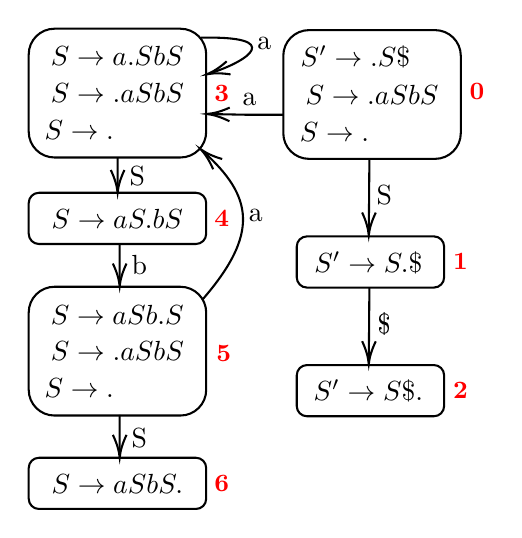
\begin{tikzpicture}[x=0.75pt,y=0.75pt,yscale=-1,xscale=1]
%Rounded Rect
\draw   (139.33,32.07) .. controls (139.33,25.22) and (144.89,19.67) .. (151.74,19.67) -- (212.44,19.67) .. controls (219.29,19.67) and (224.85,25.22) .. (224.85,32.07) -- (224.85,69.3) .. controls (224.85,76.15) and (219.29,81.71) .. (212.44,81.71) -- (151.74,81.71) .. controls (144.89,81.71) and (139.33,76.15) .. (139.33,69.3) -- cycle ;
%Rounded Rect 
\draw   (16.67,31.41) .. controls (16.67,24.56) and (22.22,19) .. (29.07,19) -- (89.77,19) .. controls (96.62,19) and (102.18,24.56) .. (102.18,31.41) -- (102.18,68.63) .. controls (102.18,75.48) and (96.62,81.04) .. (89.77,81.04) -- (29.07,81.04) .. controls (22.22,81.04) and (16.67,75.48) .. (16.67,68.63) -- cycle ;
%Rounded Rect
\draw   (16.67,155.74) .. controls (16.67,148.89) and (22.22,143.33) .. (29.07,143.33) -- (89.77,143.33) .. controls (96.62,143.33) and (102.18,148.89) .. (102.18,155.74) -- (102.18,192.97) .. controls (102.18,199.82) and (96.62,205.37) .. (89.77,205.37) -- (29.07,205.37) .. controls (22.22,205.37) and (16.67,199.82) .. (16.67,192.97) -- cycle ;
%Rounded Rect
\draw   (16.67,102.98) .. controls (16.67,100.26) and (18.88,98.05) .. (21.6,98.05) -- (97.25,98.05) .. controls (99.97,98.05) and (102.18,100.26) .. (102.18,102.98) -- (102.18,117.78) .. controls (102.18,120.51) and (99.97,122.72) .. (97.25,122.72) -- (21.6,122.72) .. controls (18.88,122.72) and (16.67,120.51) .. (16.67,117.78) -- cycle ;
%Rounded Rect
\draw   (16.67,230.65) .. controls (16.67,227.93) and (18.88,225.72) .. (21.6,225.72) -- (97.25,225.72) .. controls (99.97,225.72) and (102.18,227.93) .. (102.18,230.65) -- (102.18,245.45) .. controls (102.18,248.18) and (99.97,250.38) .. (97.25,250.38) -- (21.6,250.38) .. controls (18.88,250.38) and (16.67,248.18) .. (16.67,245.45) -- cycle ;
%Rounded Rect
\draw   (145.81,123.98) .. controls (145.81,121.26) and (148.02,119.05) .. (150.74,119.05) -- (211.87,119.05) .. controls (214.6,119.05) and (216.81,121.26) .. (216.81,123.98) -- (216.81,138.78) .. controls (216.81,141.51) and (214.6,143.72) .. (211.87,143.72) -- (150.74,143.72) .. controls (148.02,143.72) and (145.81,141.51) .. (145.81,138.78) -- cycle ;
%Rounded Rect
\draw   (145.81,185.98) .. controls (145.81,183.26) and (148.02,181.05) .. (150.74,181.05) -- (211.87,181.05) .. controls (214.6,181.05) and (216.81,183.26) .. (216.81,185.98) -- (216.81,200.78) .. controls (216.81,203.51) and (214.6,205.72) .. (211.87,205.72) -- (150.74,205.72) .. controls (148.02,205.72) and (145.81,203.51) .. (145.81,200.78) -- cycle ;
%Straight Lines 
\draw    (180.81,81.92) -- (180.53,116.51) ;
\draw [shift={(180.51,118.51)}, rotate = 270.47] [color={rgb, 255:red, 0; green, 0; blue, 0 }  ][line width=0.75]    (10.93,-3.29) .. controls (6.95,-1.4) and (3.31,-0.3) .. (0,0) .. controls (3.31,0.3) and (6.95,1.4) .. (10.93,3.29)   ;
%Straight Lines 
\draw    (180.81,143.92) -- (180.53,178.51) ;
\draw [shift={(180.51,180.51)}, rotate = 270.47] [color={rgb, 255:red, 0; green, 0; blue, 0 }  ][line width=0.75]    (10.93,-3.29) .. controls (6.95,-1.4) and (3.31,-0.3) .. (0,0) .. controls (3.31,0.3) and (6.95,1.4) .. (10.93,3.29)   ;
%Straight Lines
\draw    (59.51,81.05) -- (59.5,90) -- (59.5,96) ;
\draw [shift={(59.5,98)}, rotate = 270.03] [color={rgb, 255:red, 0; green, 0; blue, 0 }  ][line width=0.75]    (10.93,-3.29) .. controls (6.95,-1.4) and (3.31,-0.3) .. (0,0) .. controls (3.31,0.3) and (6.95,1.4) .. (10.93,3.29)   ;
%Straight Lines  
\draw    (60.51,123.05) -- (60.5,132) -- (60.5,141.08) ;
\draw [shift={(60.5,143.08)}, rotate = 270] [color={rgb, 255:red, 0; green, 0; blue, 0 }  ][line width=0.75]    (10.93,-3.29) .. controls (6.95,-1.4) and (3.31,-0.3) .. (0,0) .. controls (3.31,0.3) and (6.95,1.4) .. (10.93,3.29)   ;
%Straight Lines
\draw    (60.51,205.05) -- (60.5,214) -- (60.5,223.62) ;
\draw [shift={(60.5,225.62)}, rotate = 270.02] [color={rgb, 255:red, 0; green, 0; blue, 0 }  ][line width=0.75]    (10.93,-3.29) .. controls (6.95,-1.4) and (3.31,-0.3) .. (0,0) .. controls (3.31,0.3) and (6.95,1.4) .. (10.93,3.29)   ;
%Straight Lines
\draw    (139.5,60.47) -- (122.5,60.47) -- (104.51,60.12) ;
\draw [shift={(102.51,60.09)}, rotate = 361.09000000000003] [color={rgb, 255:red, 0; green, 0; blue, 0 }  ][line width=0.75]    (10.93,-3.29) .. controls (6.95,-1.4) and (3.31,-0.3) .. (0,0) .. controls (3.31,0.3) and (6.95,1.4) .. (10.93,3.29)   ;
%Curve Lines
\draw    (99.51,23.34) .. controls (140.25,22.37) and (122.65,34.57) .. (104.22,40.43) ;
\draw [shift={(102.51,40.96)}, rotate = 343.53999999999996] [color={rgb, 255:red, 0; green, 0; blue, 0 }  ][line width=0.75]    (10.93,-3.29) .. controls (6.95,-1.4) and (3.31,-0.3) .. (0,0) .. controls (3.31,0.3) and (6.95,1.4) .. (10.93,3.29)   ;
%Curve Lines
\draw    (100.5,149.38) .. controls (127.95,117.68) and (124.65,99.76) .. (100.98,78.35) ;
\draw [shift={(99.51,77.03)}, rotate = 401.35] [color={rgb, 255:red, 0; green, 0; blue, 0 }  ][line width=0.75]    (10.93,-3.29) .. controls (6.95,-1.4) and (3.31,-0.3) .. (0,0) .. controls (3.31,0.3) and (6.95,1.4) .. (10.93,3.29)   ;
\draw (174.09,32.69) node  [align=left] {$S' \rightarrow .S\$$};
\draw (59.33,32.33) node  [align=left] {$S \rightarrow a.SbS$};
\draw (59.33,156.67) node  [align=left] {$S \rightarrow aSb.S$};
\draw (59.33,110.67) node  [align=left] {$S \rightarrow aS.bS$};
\draw (59.33,238.33) node  [align=left] {$S \rightarrow aSbS.$};
\draw (180.33,131.67) node  [align=left] {$S' \rightarrow S.\$$};
\draw (180.33,193.67) node  [align=left] {$S' \rightarrow S\$.$};
\draw (59.42,50.02) node  [align=left] {$S \rightarrow .aSbS$};
\draw (41,68) node  [align=left] {$S \rightarrow .$};
\draw (182.09,50.69) node  [align=left] {$S \rightarrow .aSbS$};
\draw (164,69) node  [align=left] {$S \rightarrow .$};
\draw (59.42,174.35) node  [align=left] {$S \rightarrow .aSbS$};
\draw (41,192) node  [align=left] {$S \rightarrow .$};
\draw (126,109) node  [align=left] {a};
\draw (70,133) node  [align=left] {b};
\draw (123,53) node  [align=left] {a};
\draw (130,26) node  [align=left] {a};
\draw (69,90) node  [align=left] {S};
\draw (70,216) node  [align=left] {S};
\draw (188,99) node  [align=left] {S};
\draw (188,161) node  [align=left] {\$};
\draw (232.67,49.33) node  [align=left] {\textbf{{\small \textcolor{red}{0}}}};
\draw (109.67,50.33) node  [align=left] {\textbf{{\small \textcolor{red}{3}}}};
\draw (110.67,175.33) node  [align=left] {\textbf{{\small \textcolor{red}{5}}}};
\draw (224.67,131.33) node  [align=left] {\textbf{{\small \textcolor{red}{1}}}};
\draw (224.67,193.33) node  [align=left] {\textbf{{\small \textcolor{red}{2}}}};
\draw (109.67,110.33) node  [align=left] {\textbf{{\small \textcolor{red}{4}}}};
\draw (109.67,238.33) node  [align=left] {\textbf{{\small \textcolor{red}{6}}}};
\end{tikzpicture}
\end{enumerate}
\end{example}

\begin{example}
Пример управляющей таблицы для работы с построенным ранее LR-автоматом.

\begin{tabular}{|c|c|c|c||c|} 
    \hline & a & b & \$ & S \\ [0.5ex]
    \hline 0 & shift 3 & reduce 1 & reduce 1 & 1 \\
    \hline 1 & & & ACCEPT & \\
    \hline 2 & & & & \\
    \hline  3 & shift 3 & reduce 1 & reduce 1 & 4 \\
    \hline 4 & & shift 5 & & \\
    \hline 5 & shift 3 & reduce 1 & reduce 1 & 6 \\
    \hline 6 & & reduce 0 & reduce 0 & \\ [1ex] 
    \hline
\end{tabular}
\end{example}

\textbf{Ход работы LR-парсера.}
Пусть у нас есть входная строка, LR-автомат со стеком и управляющая таблица. \\
В начальный момент на стеке лежит стартовое состояние LR-автомата, позиция во входной строке соответствует её началу.
На каждом шаге анализируется текущий символ входа и текущее состояние, в котором находится автомат, и совершается одно из действий: 
\begin{itemize}
\item Если текущая позиция --- конец строки и в стеке --- стартовый нетерминал исходной грамматики, то успешно завершаем разбор.
\item Если в управляющей таблице нет инструкции для текущего состояния автомата и текущего символа на входе, то завершаем разбор с ошибкой.
\item Иначе выполняем инструкцию: \\
1) в случае shift --- кладем на стек текущий символ входа, сдвигая при этом текущую позицию, и номер нового состояния с переходом в него. \\
2) в случае reduce --- снимаем со стека 2k элементов: k состояний и k терминалов/нетерминалов (где k --- длина правой части правила, участвующего в свёртке), кладём на стек нетерминал левой части правила и, оказавшись в некотором состоянии, в котором мы были ранее (самое близкое к вершине из хранимых на стеке состояний), выполняем переход в новое состояние с добавлением его номера в стек, если в управляющей таблице пересечение текущего состояния и добавленного ранее нетерминала --- не пусто.
\end{itemize}

\begin{example}
Пример LR-разбора входного слова abab\$ из языка нашей грамматики с использованием построенных ранее LR-автомата и управляющей таблицы.
\begin{enumerate}
\item Начало разбора. На стеке --- стартовое состояние 0. \\ \\
Вход: \,
\begin{tabular}[c]{ |c|c|c|c|c| } 
    \hline \textcolor{red}{a} & b & a & b & \$ \\ \hline
\end{tabular}
\qquad Стек: \,
\begin{tabular}[c]{ |c|c } 
    \hline 0 & \\ \hline
\end{tabular}  
\\
\item Выполняем shift 3: сдвигаем указатель на входе, кладем на стек 'a', новое состояние 3 и переходим в него. \\ \\
Вход: \,
\begin{tabular}[c]{ |c|c|c|c|c| } 
    \hline a & \textcolor{red}{b} & a & b & \$ \\ \hline
\end{tabular}
\qquad Стек: \,
\begin{tabular}[c]{ |c|c|c|c } 
    \hline 0 & a & 3 & \\ \hline
\end{tabular}
\\ 
\item Выполняем reduce 1 (кладем на стек 'S'), кладем новое состояние 4 и переходим в него. \\ \\
Вход: \,
\begin{tabular}[c]{ |c|c|c|c|c| } 
    \hline a & \textcolor{red}{b} & a & b & \$ \\ \hline
\end{tabular}
\qquad Стек: \,
\begin{tabular}[c]{ |c|c|c|c|c|c } 
    \hline 0 & a & 3 & S & 4 & \\ \hline
\end{tabular}
\\ 
\item Выполняем shift 5: сдвигаем указатель на входе, кладем на стек 'b', новое состояние 5 и переходим в него. \\ \\
Вход: \,
\begin{tabular}[c]{ |c|c|c|c|c| } 
    \hline a & b & \textcolor{red}{a} & b & \$ \\ \hline
\end{tabular}
\qquad Стек: \,
\begin{tabular}[c]{ |c|c|c|c|c|c|c|c } 
    \hline 0 & a & 3 & S & 4 & b & 5 & \\ \hline
\end{tabular}
\\
\item Выполняем shift 3. \\ \\
Вход: \,
\begin{tabular}[c]{ |c|c|c|c|c| } 
    \hline a & b & a & \textcolor{red}{b} & \$ \\ \hline
\end{tabular}
\qquad Стек: \,
\begin{tabular}[c]{ |c|c|c|c|c|c|c|c|c|c } 
    \hline 0 & a & 3 & S & 4 & b & 5 & a & 3 & \\ \hline
\end{tabular}
\\
\item Выполняем reduce 1, кладем новое состояние 4 и переходим в него. \\ \\
Вход: \,
\begin{tabular}[c]{ |c|c|c|c|c| } 
    \hline a & b & a & \textcolor{red}{b} & \$ \\ \hline
\end{tabular}
\qquad Стек: \,
\begin{tabular}[c]{ |c|c|c|c|c|c|c|c|c|c|c|c } 
    \hline 0 & a & 3 & S & 4 & b & 5 & a & 3 & S & 4 & \\ \hline
\end{tabular}
\\
\item Выполняем shift 5. \\ \\
Вход: \,
\begin{tabular}[c]{ |c|c|c|c|c| } 
    \hline a & b & a & b & \textcolor{red}{\$} \\ \hline
\end{tabular}
\qquad Стек: \,
\begin{tabular}[c]{ |c|c|c|c|c|c|c|c|c|c|c|c|c|c } 
    \hline 0 & a & 3 & S & 4 & b & 5 & a & 3 & S & 4 & b & 5 & \\ \hline
\end{tabular}
\\
\item Выполняем reduce 1, кладем новое состояние 6 и переходим в него. \\ \\
Вход: \,
\begin{tabular}[c]{ |c|c|c|c|c| } 
    \hline a & b & a & b & \textcolor{red}{\$} \\ \hline
\end{tabular}
\qquad Стек: \,
\begin{tabular}[c]{ |c|c|c|c|c|c|c|c|c|c|c|c|c|c|c|c } 
    \hline 0 & a & 3 & S & 4 & b & 5 & a & 3 & S & 4 & b & 5 & S & 6 & \\ \hline
\end{tabular}
\\
\item Выполняем reduce 0 (снимаем со стека 8 элементов и кладем 'S'), оказываемся в состоянии 5 и делаем переход в новое состояние 6 с добавлением его на стек. \\ \\
Вход: \,
\begin{tabular}[c]{ |c|c|c|c|c| } 
    \hline a & b & a & b & \textcolor{red}{\$} \\ \hline
\end{tabular}
\qquad Стек: \,
\begin{tabular}[c]{ |c|c|c|c|c|c|c|c|c|c } 
    \hline 0 & a & 3 & S & 4 & b & 5 & S & 6 & \\ \hline
\end{tabular}
\\
\item Снова выполняем reduce 0, оказываемся в состоянии 0 и делаем переход в новое состояние 1 с добавлением его на стек. Заканчиваем разбор. \\ \\
Вход: \,
\begin{tabular}[c]{ |c|c|c|c|c| } 
    \hline a & b & a & b & \textcolor{red}{\$} \\ \hline
\end{tabular}
\qquad Стек: \,
\begin{tabular}[c]{ |c|c|c|c } 
    \hline 0 & S & 1 & \\ \hline
\end{tabular}
\end{enumerate}
\end{example}

На практике конфликты стараются решать ещё и на этапе генерации.
Да, реальные тулы могут сгенерировать парсер по неоднозначной грамматике: из переноса или свёртки выбирать перенос, из нескольких свёрток --- первую в каком-то порядке (обычно в порядке появления соответствующих продукций в грамматике).

Существует также модификация LR-разбора, которая называется SLR (Simple LR). 
Основная идея заключается в том, чтобы хранить в управляющей таблице reduce-инструкции только для тех терминалов, которые встречаются в правилах грамматики сразу после нетерминала, к которому выполняется свертка. 
Также существует LALR модификация (Look-Ahead LR).
В ней применяется склеивание нескольких состояний автомата, входные дуги которых имеют общие символы переходы, в одно состояние.
Данные модификации позволяют избежать большее число конфликтов, однако иногда могут иметь таблицы большего размера, чем в классическом LR.
Стоит отметить, что LALR(1)-парсер --- менее мощный, чем LR(1)-парсер, но более мощный, чем SLR(1)-парсер.

\section{GLR и его применение для КС запросов}

Алгоритм LR довольно эффективен, однако позволяет работать не со всеми КС-грамматиками, а только с их подмножеством LR(k). Если грамматика находится за рамками допускаемого класса, некоторые ячейки управляющей таблицы могут содержать несколько значений. В этом случае грамматика отвергалась анализатором.

Чтобы допустить множестенные значения в ячейках управляющей таблицы, потребуется некоторый вид недетерминизма, который даст возможность анализатору обрабатывать несколько возможных вариантов синтаксического разбора параллельно. Именно это и предлагает анализатор Generalized LR (GLR)~\cite{tomita-1987-efficient}. Далее мы рассмотрим общий принцип работы, проиллюстрируем его с помощью примера, а также рассмотрим модификации GLR.

\subsection{Классический GLR алгоритм}

Впервые GLR парсер был представлен Масару Томитой в 1987~\cite{tomita-1987-efficient}. В целом, алгоритм работы идентичен LR с несколькими принципиальными исключениями:
\begin{itemize}
    \item Управляющая таблица модифицирована таким образом, чтобы допускать множественные значения в ячейках.
    \item Для каждой операции reduce, которую мы можем применить на каком-то этапе разбора, создается копия всего стека, после чего, к ней применяется эта операция.
    \item Если к стеку нельзя применить ни одну операцию shift на следующем входном символе, то этот стек отбрасывается.
\end{itemize}

Однако, полное копирование стеков приводит к тому, что дублируется слишком много информации. Поэтому можно сделать следующее:
\begin{itemize}
    \item Объединять одинаковые состояния.
    \item Объединять одинаковые правые префиксы стеков (то есть верхние их части, к которым быстрее всего доберутся операции reduce).
\end{itemize}

Для этого стоит использовать более сложную структуру стека: \textit{граф-структурированный стек} или (\textit{GSS}, Graph Structured Stack). Это направленный граф, в котором вершины соответствуют элементам стека, а ребра их соединяют по правилам управляющей таблицы. У каждой вершины может быть несколько входящих и исходящих узлов: таким образом реализуется то самое объединение, упомянутое в предыдущем абзаце.

\begin{example}
    \label{glr:example}
    Рассмотрим пример GLR разбора с использованием GSS.
    
    Возьмем грамматику $G$ следующего вида:
    \begin{align*}
        &0.\quad S' \to S\$ \\
        &1.\quad S \to abC \\
        &2.\quad S \to aBC \\
        &3.\quad B \to b \\
        &4.\quad C \to c 
    \end{align*}
    
    Входное слово $ w $:
    \begin{align*}
        w = abc\$
    \end{align*}
    
    Построим для данной грамматики LR автомат:
    
    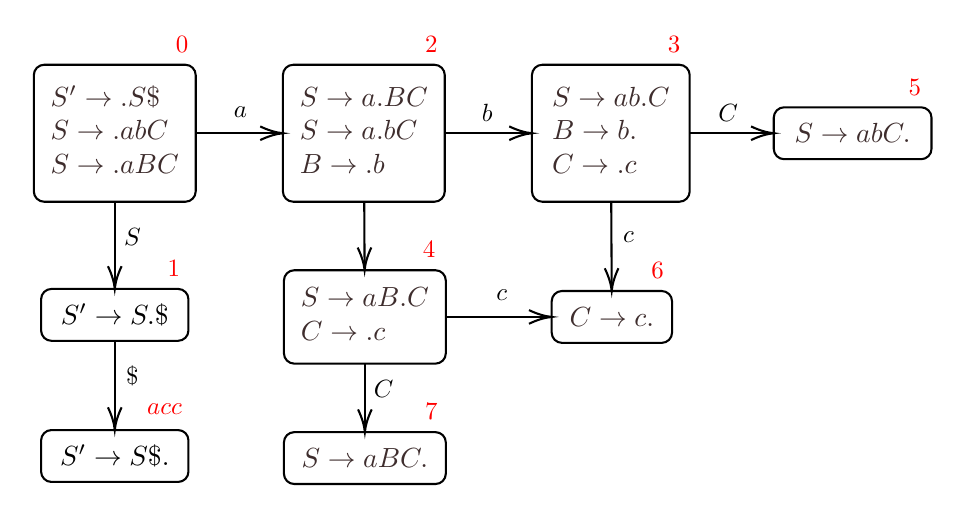
\begin{tikzpicture}[x=0.75pt,y=0.75pt,yscale=-1,xscale=1]
    %uncomment if require: \path (0,306); %set diagram left start at 0, and has height of 306
    
    
    % Text Node
    \draw    (21.5,33) .. controls (21.5,30.24) and (23.74,28) .. (26.5,28) -- (94.5,28) .. controls (97.26,28) and (99.5,30.24) .. (99.5,33) -- (99.5,89) .. controls (99.5,91.76) and (97.26,94) .. (94.5,94) -- (26.5,94) .. controls (23.74,94) and (21.5,91.76) .. (21.5,89) -- cycle  ;
    \draw (60.5,61) node [color={rgb, 255:red, 62; green, 45; blue, 45 }  ,opacity=1 ]  {$ \begin{array}{l}
        S'\rightarrow .S\$\\
        S\rightarrow .abC\\
        S\rightarrow .aBC
        \end{array}$};
    % Text Node
    \draw    (25,141) .. controls (25,138.24) and (27.24,136) .. (30,136) -- (91,136) .. controls (93.76,136) and (96,138.24) .. (96,141) -- (96,156) .. controls (96,158.76) and (93.76,161) .. (91,161) -- (30,161) .. controls (27.24,161) and (25,158.76) .. (25,156) -- cycle  ;
    \draw (60.5,148.5) node   {$S'\rightarrow S.\$$};
    % Text Node
    \draw (446,39) node [scale=0.9,color={rgb, 255:red, 255; green, 0; blue, 0 }  ,opacity=1 ]  {$5$};
    % Text Node
    \draw (93,18) node [scale=0.9,color={rgb, 255:red, 255; green, 0; blue, 0 }  ,opacity=1 ]  {$0$};
    % Text Node
    \draw (213,18) node [scale=0.9,color={rgb, 255:red, 255; green, 0; blue, 0 }  ,opacity=1 ]  {$2$};
    % Text Node
    \draw (89,126) node [scale=0.9,color={rgb, 255:red, 255; green, 0; blue, 0 }  ,opacity=1 ]  {$1$};
    % Text Node
    \draw (330,18) node [scale=0.9,color={rgb, 255:red, 255; green, 0; blue, 0 }  ,opacity=1 ]  {$3$};
    % Text Node
    \draw (212,117) node [scale=0.9,color={rgb, 255:red, 255; green, 0; blue, 0 }  ,opacity=1 ]  {$4$};
    % Text Node
    \draw    (141.5,33) .. controls (141.5,30.24) and (143.74,28) .. (146.5,28) -- (214.5,28) .. controls (217.26,28) and (219.5,30.24) .. (219.5,33) -- (219.5,89) .. controls (219.5,91.76) and (217.26,94) .. (214.5,94) -- (146.5,94) .. controls (143.74,94) and (141.5,91.76) .. (141.5,89) -- cycle  ;
    \draw (180.5,61) node [color={rgb, 255:red, 62; green, 45; blue, 45 }  ,opacity=1 ]  {$ \begin{array}{l}
        S\rightarrow a.BC\\
        S\rightarrow a.bC\\
        B\rightarrow .b
        \end{array}$};
    % Text Node
    \draw (121,51) node [scale=0.9,color={rgb, 255:red, 0; green, 0; blue, 0 }  ,opacity=1 ]  {$a$};
    % Text Node
    \draw    (261.5,33) .. controls (261.5,30.24) and (263.74,28) .. (266.5,28) -- (332.5,28) .. controls (335.26,28) and (337.5,30.24) .. (337.5,33) -- (337.5,89) .. controls (337.5,91.76) and (335.26,94) .. (332.5,94) -- (266.5,94) .. controls (263.74,94) and (261.5,91.76) .. (261.5,89) -- cycle  ;
    \draw (299.5,61) node [color={rgb, 255:red, 62; green, 45; blue, 45 }  ,opacity=1 ]  {$ \begin{array}{l}
        S\rightarrow ab.C\\
        B\rightarrow b.\\
        C\rightarrow .c
        \end{array}$};
    % Text Node
    \draw    (25,209) .. controls (25,206.24) and (27.24,204) .. (30,204) -- (91,204) .. controls (93.76,204) and (96,206.24) .. (96,209) -- (96,224) .. controls (96,226.76) and (93.76,229) .. (91,229) -- (30,229) .. controls (27.24,229) and (25,226.76) .. (25,224) -- cycle  ;
    \draw (60.5,216.5) node   {$S'\rightarrow S\$.$};
    % Text Node
    \draw (69,111) node [scale=0.9,color={rgb, 255:red, 0; green, 0; blue, 0 }  ,opacity=1 ]  {$S$};
    % Text Node
    \draw (69,178) node [scale=0.9,color={rgb, 255:red, 0; green, 0; blue, 0 }  ,opacity=1 ]  {$\$$};
    % Text Node
    \draw    (378,53.5) .. controls (378,50.74) and (380.24,48.5) .. (383,48.5) -- (449,48.5) .. controls (451.76,48.5) and (454,50.74) .. (454,53.5) -- (454,68.5) .. controls (454,71.26) and (451.76,73.5) .. (449,73.5) -- (383,73.5) .. controls (380.24,73.5) and (378,71.26) .. (378,68.5) -- cycle  ;
    \draw (416,61) node [color={rgb, 255:red, 62; green, 45; blue, 45 }  ,opacity=1 ]  {$S\rightarrow abC.$};
    % Text Node
    \draw (240,51) node [scale=0.9,color={rgb, 255:red, 0; green, 0; blue, 0 }  ,opacity=1 ]  {$b$};
    % Text Node
    \draw (356,51) node [scale=0.9,color={rgb, 255:red, 0; green, 0; blue, 0 }  ,opacity=1 ]  {$C$};
    % Text Node
    \draw    (142,132) .. controls (142,129.24) and (144.24,127) .. (147,127) -- (215,127) .. controls (217.76,127) and (220,129.24) .. (220,132) -- (220,167) .. controls (220,169.76) and (217.76,172) .. (215,172) -- (147,172) .. controls (144.24,172) and (142,169.76) .. (142,167) -- cycle  ;
    \draw (181,149.5) node [color={rgb, 255:red, 62; green, 45; blue, 45 }  ,opacity=1 ]  {$ \begin{array}{l}
        S\rightarrow aB.C\\
        C\rightarrow .c
        \end{array}$};
    % Text Node
    \draw    (142,210) .. controls (142,207.24) and (144.24,205) .. (147,205) -- (215,205) .. controls (217.76,205) and (220,207.24) .. (220,210) -- (220,225) .. controls (220,227.76) and (217.76,230) .. (215,230) -- (147,230) .. controls (144.24,230) and (142,227.76) .. (142,225) -- cycle  ;
    \draw (181,217.5) node [color={rgb, 255:red, 62; green, 45; blue, 45 }  ,opacity=1 ]  {$S\rightarrow aBC.$};
    % Text Node
    \draw    (271,142) .. controls (271,139.24) and (273.24,137) .. (276,137) -- (324,137) .. controls (326.76,137) and (329,139.24) .. (329,142) -- (329,157) .. controls (329,159.76) and (326.76,162) .. (324,162) -- (276,162) .. controls (273.24,162) and (271,159.76) .. (271,157) -- cycle  ;
    \draw (300,149.5) node [color={rgb, 255:red, 62; green, 45; blue, 45 }  ,opacity=1 ]  {$C\rightarrow c.$};
    % Text Node
    \draw (247,139) node [scale=0.9,color={rgb, 255:red, 0; green, 0; blue, 0 }  ,opacity=1 ]  {$c$};
    % Text Node
    \draw (308,111) node [scale=0.9,color={rgb, 255:red, 0; green, 0; blue, 0 }  ,opacity=1 ]  {$c$};
    % Text Node
    \draw (190,184) node [scale=0.9,color={rgb, 255:red, 0; green, 0; blue, 0 }  ,opacity=1 ]  {$C$};
    % Text Node
    \draw (322,127) node [scale=0.9,color={rgb, 255:red, 255; green, 0; blue, 0 }  ,opacity=1 ]  {$6$};
    % Text Node
    \draw (213,195) node [scale=0.9,color={rgb, 255:red, 255; green, 0; blue, 0 }  ,opacity=1 ]  {$7$};
    % Text Node
    \draw (84.5,194) node [scale=0.9,color={rgb, 255:red, 255; green, 0; blue, 0 }  ,opacity=1 ]  {$acc$};
    % Connection
    \draw    (99.5,61) -- (139.5,61) ;
    \draw [shift={(141.5,61)}, rotate = 180] [color={rgb, 255:red, 0; green, 0; blue, 0 }  ][line width=0.75]    (10.93,-3.29) .. controls (6.95,-1.4) and (3.31,-0.3) .. (0,0) .. controls (3.31,0.3) and (6.95,1.4) .. (10.93,3.29)   ;
    
    % Connection
    \draw    (60.5,94) -- (60.5,134) ;
    \draw [shift={(60.5,136)}, rotate = 270] [color={rgb, 255:red, 0; green, 0; blue, 0 }  ][line width=0.75]    (10.93,-3.29) .. controls (6.95,-1.4) and (3.31,-0.3) .. (0,0) .. controls (3.31,0.3) and (6.95,1.4) .. (10.93,3.29)   ;
    
    % Connection
    \draw    (60.5,161) -- (60.5,202) ;
    \draw [shift={(60.5,204)}, rotate = 270] [color={rgb, 255:red, 0; green, 0; blue, 0 }  ][line width=0.75]    (10.93,-3.29) .. controls (6.95,-1.4) and (3.31,-0.3) .. (0,0) .. controls (3.31,0.3) and (6.95,1.4) .. (10.93,3.29)   ;
    
    % Connection
    \draw    (219.5,61) -- (259.5,61) ;
    \draw [shift={(261.5,61)}, rotate = 180] [color={rgb, 255:red, 0; green, 0; blue, 0 }  ][line width=0.75]    (10.93,-3.29) .. controls (6.95,-1.4) and (3.31,-0.3) .. (0,0) .. controls (3.31,0.3) and (6.95,1.4) .. (10.93,3.29)   ;
    
    % Connection
    \draw    (337.5,61) -- (376,61) ;
    \draw [shift={(378,61)}, rotate = 180] [color={rgb, 255:red, 0; green, 0; blue, 0 }  ][line width=0.75]    (10.93,-3.29) .. controls (6.95,-1.4) and (3.31,-0.3) .. (0,0) .. controls (3.31,0.3) and (6.95,1.4) .. (10.93,3.29)   ;
    
    % Connection
    \draw    (180.69,94) -- (180.86,125) ;
    \draw [shift={(180.87,127)}, rotate = 269.68] [color={rgb, 255:red, 0; green, 0; blue, 0 }  ][line width=0.75]    (10.93,-3.29) .. controls (6.95,-1.4) and (3.31,-0.3) .. (0,0) .. controls (3.31,0.3) and (6.95,1.4) .. (10.93,3.29)   ;
    
    % Connection
    \draw    (181,172) -- (181,203) ;
    \draw [shift={(181,205)}, rotate = 270] [color={rgb, 255:red, 0; green, 0; blue, 0 }  ][line width=0.75]    (10.93,-3.29) .. controls (6.95,-1.4) and (3.31,-0.3) .. (0,0) .. controls (3.31,0.3) and (6.95,1.4) .. (10.93,3.29)   ;
    
    % Connection
    \draw    (299.69,94) -- (299.92,135) ;
    \draw [shift={(299.93,137)}, rotate = 269.68] [color={rgb, 255:red, 0; green, 0; blue, 0 }  ][line width=0.75]    (10.93,-3.29) .. controls (6.95,-1.4) and (3.31,-0.3) .. (0,0) .. controls (3.31,0.3) and (6.95,1.4) .. (10.93,3.29)   ;
    
    % Connection
    \draw    (220,149.5) -- (269,149.5) ;
    \draw [shift={(271,149.5)}, rotate = 180] [color={rgb, 255:red, 0; green, 0; blue, 0 }  ][line width=0.75]    (10.93,-3.29) .. controls (6.95,-1.4) and (3.31,-0.3) .. (0,0) .. controls (3.31,0.3) and (6.95,1.4) .. (10.93,3.29)   ;
    
    
    \end{tikzpicture}
    
    И управляющую таблицу:
    
    \begin{tabular}{|c|c|c|c|c||c|c|c|} 
        \hline   & a & b & c & \$ & B & C & S \\ [0.5ex]
        \hline 0 & shift 2 & & & & & goto 1 & \\
        \hline 1 &   &   &   &  accept  &   &   & \\
        \hline 2 &   & shift 3  &   &    & goto 4  &   & \\
        \hline 3 &   &   & shift 6 OR reduce 3  &    &   & goto 5  & \\
        \hline 4 &   &   & shift 6  &    &   & goto 7  & \\
        \hline 5 &   &   &   & reduce 1   &   &   & \\
        \hline 6 &   &   &   & reduce 4   &   &   & \\
        \hline 7 &   &   &   & reduce 2   &   &   & \\ [1ex] 
        \hline
    \end{tabular}
    
    Разберем слово $w$ с помощью алгоритма GLR. Использована следующая аннотация: вершины-состояния обозначены кругами, вершины-символы --- прямоугольниками.
    \begin{enumerate}
        \item Инициализируем GSS стартовым состоянием $v_0$: \\ \\
        Вход: \,
        \begin{tabular}[c]{ |c|c|c|c| } 
            \hline a & b & c & \$ \\ \hline
        \end{tabular}
        \qquad GSS: \,
        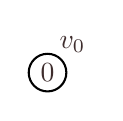
\begin{tikzpicture}[x=0.5pt,y=0.5pt,yscale=-1,xscale=1]
        %uncomment if require: \path (0,306); %set diagram left start at 0, and has height of 306
        
        
        % Text Node
        \draw  [line width=0.75]   (92, 109) circle [x radius= 13.6, y radius= 13.6]   ;
        \draw (92,109) node [color={rgb, 255:red, 62; green, 45; blue, 45 }  ,opacity=1 ]  {$0$};
        % Text Node
        \draw (110,89) node [color={rgb, 255:red, 62; green, 45; blue, 45 }  ,opacity=1 ]  {$v_{0}$};
        
        
        \end{tikzpicture}
        \\
        
        \item Видим входной символ '$a$', ищем соответствующую ему операцию в управляющей таблице --- $shift\ 2$, строим новый узел $v_1$: \\ \\
        Вход: \,
        \begin{tabular}[c]{ |c|c|c|c| } 
            \hline \textcolor{red}{a} & b & c & \$ \\ \hline
        \end{tabular}
        \qquad GSS: \,
        \begin{tikzpicture}[x=0.5pt,y=0.5pt,yscale=-1,xscale=1]
        %uncomment if require: \path (0,306); %set diagram left start at 0, and has height of 306
        
        
        % Text Node
        \draw  [line width=0.75]   (92, 109) circle [x radius= 13.6, y radius= 13.6]   ;
        \draw (92,109) node [color={rgb, 255:red, 62; green, 45; blue, 45 }  ,opacity=1 ]  {$0$};
        % Text Node
        \draw  [line width=0.75]   (138,98) -- (156,98) -- (156,122) -- (138,122) -- cycle  ;
        \draw (147,110) node [scale=1,color={rgb, 255:red, 62; green, 45; blue, 45 }  ,opacity=1 ]  {а};
        % Text Node
        \draw  [line width=0.75]   (203, 110) circle [x radius= 13.6, y radius= 13.6]   ;
        \draw (203,110) node [color={rgb, 255:red, 62; green, 45; blue, 45 }  ,opacity=1 ]  {$2$};
        % Text Node
        \draw (110,89) node [color={rgb, 255:red, 62; green, 45; blue, 45 }  ,opacity=1 ]  {$v_{0}$};
        % Text Node
        \draw (220,89) node [color={rgb, 255:red, 62; green, 45; blue, 45 }  ,opacity=1 ]  {$v_{1}$};
        % Connection
        \draw    (138,109.84) -- (107.6,109.28) ;
        \draw [shift={(105.6,109.25)}, rotate = 361.03999999999996] [color={rgb, 255:red, 0; green, 0; blue, 0 }  ][line width=0.75]    (10.93,-3.29) .. controls (6.95,-1.4) and (3.31,-0.3) .. (0,0) .. controls (3.31,0.3) and (6.95,1.4) .. (10.93,3.29)   ;
        
        % Connection
        \draw    (189.4,110) -- (158,110) ;
        \draw [shift={(156,110)}, rotate = 360] [color={rgb, 255:red, 0; green, 0; blue, 0 }  ][line width=0.75]    (10.93,-3.29) .. controls (6.95,-1.4) and (3.31,-0.3) .. (0,0) .. controls (3.31,0.3) and (6.95,1.4) .. (10.93,3.29)   ;
        
        
        \end{tikzpicture}
        \\
        
        \item Повторяем для символа '$b$', операции $shift\ 3$ и узла $v_2$: \\ \\
        Вход: \,
        \begin{tabular}[c]{ |c|c|c|c| } 
            \hline a & \textcolor{red}{b} & c & \$ \\ \hline
        \end{tabular}
        \qquad GSS: \,
        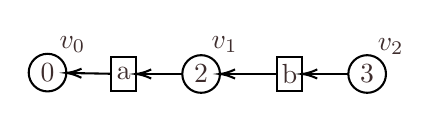
\begin{tikzpicture}[x=0.5pt,y=0.5pt,yscale=-1,xscale=1]
        %uncomment if require: \path (0,306); %set diagram left start at 0, and has height of 306
        
        
        % Text Node
        \draw  [line width=0.75]   (92, 109) circle [x radius= 13.6, y radius= 13.6]   ;
        \draw (92,109) node [color={rgb, 255:red, 62; green, 45; blue, 45 }  ,opacity=1 ]  {$0$};
        % Text Node
        \draw  [line width=0.75]   (138,98) -- (156,98) -- (156,122) -- (138,122) -- cycle  ;
        \draw (147,110) node [scale=1,color={rgb, 255:red, 62; green, 45; blue, 45 }  ,opacity=1 ]  {a};
        % Text Node
        \draw  [line width=0.75]   (203, 110) circle [x radius= 13.6, y radius= 13.6]   ;
        \draw (203,110) node [color={rgb, 255:red, 62; green, 45; blue, 45 }  ,opacity=1 ]  {$2$};
        % Text Node
        \draw (110,89) node [color={rgb, 255:red, 62; green, 45; blue, 45 }  ,opacity=1 ]  {$v_{0}$};
        % Text Node
        \draw (220,89) node [color={rgb, 255:red, 62; green, 45; blue, 45 }  ,opacity=1 ]  {$v_{1}$};
        % Text Node
        \draw  [line width=0.75]   (258,98) -- (276,98) -- (276,122) -- (258,122) -- cycle  ;
        \draw (267,110) node [scale=1,color={rgb, 255:red, 62; green, 45; blue, 45 }  ,opacity=1 ]  {b};
        % Text Node
        \draw  [line width=0.75]   (323, 110) circle [x radius= 13.6, y radius= 13.6]   ;
        \draw (323,110) node [color={rgb, 255:red, 62; green, 45; blue, 45 }  ,opacity=1 ]  {$3$};
        % Text Node
        \draw (340,90) node [color={rgb, 255:red, 62; green, 45; blue, 45 }  ,opacity=1 ]  {$v_{2}$};
        % Connection
        \draw    (138,109.84) -- (107.6,109.28) ;
        \draw [shift={(105.6,109.25)}, rotate = 361.03999999999996] [color={rgb, 255:red, 0; green, 0; blue, 0 }  ][line width=0.75]    (10.93,-3.29) .. controls (6.95,-1.4) and (3.31,-0.3) .. (0,0) .. controls (3.31,0.3) and (6.95,1.4) .. (10.93,3.29)   ;
        
        % Connection
        \draw    (189.4,110) -- (158,110) ;
        \draw [shift={(156,110)}, rotate = 360] [color={rgb, 255:red, 0; green, 0; blue, 0 }  ][line width=0.75]    (10.93,-3.29) .. controls (6.95,-1.4) and (3.31,-0.3) .. (0,0) .. controls (3.31,0.3) and (6.95,1.4) .. (10.93,3.29)   ;
        
        % Connection
        \draw    (309.4,110) -- (278,110) ;
        \draw [shift={(276,110)}, rotate = 360] [color={rgb, 255:red, 0; green, 0; blue, 0 }  ][line width=0.75]    (10.93,-3.29) .. controls (6.95,-1.4) and (3.31,-0.3) .. (0,0) .. controls (3.31,0.3) and (6.95,1.4) .. (10.93,3.29)   ;
        
        % Connection
        \draw    (258,110) -- (218.6,110) ;
        \draw [shift={(216.6,110)}, rotate = 360] [color={rgb, 255:red, 0; green, 0; blue, 0 }  ][line width=0.75]    (10.93,-3.29) .. controls (6.95,-1.4) and (3.31,-0.3) .. (0,0) .. controls (3.31,0.3) and (6.95,1.4) .. (10.93,3.29)   ;
        
        
        \end{tikzpicture}
        \\
        
        \item При обработке узла $v_3$ у нас возникает конфликт shift-reduce: $shift\ 6\ OR\ reduce\ 3$. Мы смотрим на вершины, смежные $v_2$, на управляющую таблицу и на правило вывода под номером 3 для поиска альтернативного построения стека. Находим $goto\ 4$ и строим вершину $v_3$ с соответствующим переходом по нетерминалу $B$ из $v_1$ (т.к. количество символов в правой части правила вывода 3 равняется 1, значит мы в дереве опустимся на глубину 1 по вершинам-состояниям):\\ \\
        Вход: \,
        \begin{tabular}[c]{ |c|c|c|c| } 
            \hline a & b & c & \$ \\ \hline
        \end{tabular}
        \qquad GSS: \,
        \begin{tikzpicture}[x=0.5pt,y=0.5pt,yscale=-1,xscale=1]
        %uncomment if require: \path (0,422); %set diagram left start at 0, and has height of 422
        
        
        % Text Node
        \draw  [line width=0.75]   (92, 110) circle [x radius= 13.6, y radius= 13.6]   ;
        \draw (92,110) node [color={rgb, 255:red, 62; green, 45; blue, 45 }  ,opacity=1 ]  {$0$};
        % Text Node
        \draw  [line width=0.75]   (138,98) -- (156,98) -- (156,122) -- (138,122) -- cycle  ;
        \draw (147,110) node [scale=1,color={rgb, 255:red, 62; green, 45; blue, 45 }  ,opacity=1 ]  {а};
        % Text Node
        \draw  [line width=0.75]   (203, 110) circle [x radius= 13.6, y radius= 13.6]   ;
        \draw (203,110) node [color={rgb, 255:red, 62; green, 45; blue, 45 }  ,opacity=1 ]  {$2$};
        % Text Node
        \draw (110,89) node [color={rgb, 255:red, 62; green, 45; blue, 45 }  ,opacity=1 ]  {$v_{0}$};
        % Text Node
        \draw (220,89) node [color={rgb, 255:red, 62; green, 45; blue, 45 }  ,opacity=1 ]  {$v_{1}$};
        % Text Node
        \draw  [line width=0.75]   (258,98) -- (276,98) -- (276,122) -- (258,122) -- cycle  ;
        \draw (267,110) node [scale=1,color={rgb, 255:red, 62; green, 45; blue, 45 }  ,opacity=1 ]  {b};
        % Text Node
        \draw  [line width=0.75]   (323, 110) circle [x radius= 13.6, y radius= 13.6]   ;
        \draw (323,110) node [color={rgb, 255:red, 62; green, 45; blue, 45 }  ,opacity=1 ]  {$3$};
        % Text Node
        \draw (340,90) node [color={rgb, 255:red, 62; green, 45; blue, 45 }  ,opacity=1 ]  {$v_{2}$};
        % Text Node
        \draw  [line width=0.75]   (258,158) -- (276,158) -- (276,182) -- (258,182) -- cycle  ;
        \draw (267,170) node [scale=1,color={rgb, 255:red, 62; green, 45; blue, 45 }  ,opacity=1 ]  {B};
        % Text Node
        \draw  [line width=0.75]   (323, 170) circle [x radius= 13.6, y radius= 13.6]   ;
        \draw (323,170) node [color={rgb, 255:red, 62; green, 45; blue, 45 }  ,opacity=1 ]  {$4$};
        % Text Node
        \draw (340,149) node [color={rgb, 255:red, 62; green, 45; blue, 45 }  ,opacity=1 ]  {$v_{3}$};
        % Connection
        \draw    (138,110) -- (107.6,110) ;
        \draw [shift={(105.6,110)}, rotate = 360] [color={rgb, 255:red, 0; green, 0; blue, 0 }  ][line width=0.75]    (10.93,-3.29) .. controls (6.95,-1.4) and (3.31,-0.3) .. (0,0) .. controls (3.31,0.3) and (6.95,1.4) .. (10.93,3.29)   ;
        
        % Connection
        \draw    (189.4,110) -- (158,110) ;
        \draw [shift={(156,110)}, rotate = 360] [color={rgb, 255:red, 0; green, 0; blue, 0 }  ][line width=0.75]    (10.93,-3.29) .. controls (6.95,-1.4) and (3.31,-0.3) .. (0,0) .. controls (3.31,0.3) and (6.95,1.4) .. (10.93,3.29)   ;
        
        % Connection
        \draw    (309.4,110) -- (278,110) ;
        \draw [shift={(276,110)}, rotate = 360] [color={rgb, 255:red, 0; green, 0; blue, 0 }  ][line width=0.75]    (10.93,-3.29) .. controls (6.95,-1.4) and (3.31,-0.3) .. (0,0) .. controls (3.31,0.3) and (6.95,1.4) .. (10.93,3.29)   ;
        
        % Connection
        \draw    (258,110) -- (218.6,110) ;
        \draw [shift={(216.6,110)}, rotate = 360] [color={rgb, 255:red, 0; green, 0; blue, 0 }  ][line width=0.75]    (10.93,-3.29) .. controls (6.95,-1.4) and (3.31,-0.3) .. (0,0) .. controls (3.31,0.3) and (6.95,1.4) .. (10.93,3.29)   ;
        
        % Connection
        \draw    (309.4,170) -- (278,170) ;
        \draw [shift={(276,170)}, rotate = 360] [color={rgb, 255:red, 0; green, 0; blue, 0 }  ][line width=0.75]    (10.93,-3.29) .. controls (6.95,-1.4) and (3.31,-0.3) .. (0,0) .. controls (3.31,0.3) and (6.95,1.4) .. (10.93,3.29)   ;
        
        % Connection
        \draw    (258,168.07) .. controls (230.15,163.58) and (213.3,149.18) .. (207.42,124.89) ;
        \draw [shift={(206.99,123.01)}, rotate = 437.91] [color={rgb, 255:red, 0; green, 0; blue, 0 }  ][line width=0.75]    (10.93,-3.29) .. controls (6.95,-1.4) and (3.31,-0.3) .. (0,0) .. controls (3.31,0.3) and (6.95,1.4) .. (10.93,3.29)   ;
        
        
        \end{tikzpicture}
        \\
        
        \item Читаем символ '$c$' и ищем в управляющей таблице переходы из состояний 3 и 4 (так как узлы $v_2$ и $v_3$ находятся на одном уровне, то есть были построены после чтения одного символа из входного слова). Таким переходом оказывается $shift\ 6$ в обоих случаях, поэтому соединяем узел $v_4$ с обоими рассмотренными узлами:\\ \\
        Вход: \,
        \begin{tabular}[c]{ |c|c|c|c| } 
            \hline a & b & \textcolor{red}{c} & \$ \\ \hline
        \end{tabular}
        \qquad GSS: \,
        \begin{tikzpicture}[x=0.5pt,y=0.5pt,yscale=-1,xscale=1]
        %uncomment if require: \path (0,422); %set diagram left start at 0, and has height of 422
        
        
        % Text Node
        \draw  [line width=0.75]   (92, 110) circle [x radius= 13.6, y radius= 13.6]   ;
        \draw (92,110) node [color={rgb, 255:red, 62; green, 45; blue, 45 }  ,opacity=1 ]  {$0$};
        % Text Node
        \draw  [line width=0.75]   (138,98) -- (156,98) -- (156,122) -- (138,122) -- cycle  ;
        \draw (147,110) node [scale=1,color={rgb, 255:red, 62; green, 45; blue, 45 }  ,opacity=1 ]  {а};
        % Text Node
        \draw  [line width=0.75]   (203, 110) circle [x radius= 13.6, y radius= 13.6]   ;
        \draw (203,110) node [color={rgb, 255:red, 62; green, 45; blue, 45 }  ,opacity=1 ]  {$2$};
        % Text Node
        \draw (110,89) node [color={rgb, 255:red, 62; green, 45; blue, 45 }  ,opacity=1 ]  {$v_{0}$};
        % Text Node
        \draw (220,89) node [color={rgb, 255:red, 62; green, 45; blue, 45 }  ,opacity=1 ]  {$v_{1}$};
        % Text Node
        \draw  [line width=0.75]   (258,98) -- (276,98) -- (276,122) -- (258,122) -- cycle  ;
        \draw (267,110) node [scale=1,color={rgb, 255:red, 62; green, 45; blue, 45 }  ,opacity=1 ]  {b};
        % Text Node
        \draw  [line width=0.75]   (323, 110) circle [x radius= 13.6, y radius= 13.6]   ;
        \draw (323,110) node [color={rgb, 255:red, 62; green, 45; blue, 45 }  ,opacity=1 ]  {$3$};
        % Text Node
        \draw (340,90) node [color={rgb, 255:red, 62; green, 45; blue, 45 }  ,opacity=1 ]  {$v_{2}$};
        % Text Node
        \draw  [line width=0.75]   (258,158) -- (276,158) -- (276,182) -- (258,182) -- cycle  ;
        \draw (267,170) node [scale=1,color={rgb, 255:red, 62; green, 45; blue, 45 }  ,opacity=1 ]  {B};
        % Text Node
        \draw  [line width=0.75]   (323, 170) circle [x radius= 13.6, y radius= 13.6]   ;
        \draw (323,170) node [color={rgb, 255:red, 62; green, 45; blue, 45 }  ,opacity=1 ]  {$4$};
        % Text Node
        \draw (340,149) node [color={rgb, 255:red, 62; green, 45; blue, 45 }  ,opacity=1 ]  {$v_{3}$};
        % Text Node
        \draw  [line width=0.75]   (374,98) -- (392,98) -- (392,122) -- (374,122) -- cycle  ;
        \draw (383,110) node [scale=1,color={rgb, 255:red, 62; green, 45; blue, 45 }  ,opacity=1 ]  {c};
        % Text Node
        \draw  [line width=0.75]   (374,158) -- (392,158) -- (392,182) -- (374,182) -- cycle  ;
        \draw (383,170) node [scale=1,color={rgb, 255:red, 62; green, 45; blue, 45 }  ,opacity=1 ]  {c};
        % Text Node
        \draw  [line width=0.75]   (437, 110) circle [x radius= 13.6, y radius= 13.6]   ;
        \draw (437,110) node [color={rgb, 255:red, 62; green, 45; blue, 45 }  ,opacity=1 ]  {$6$};
        % Text Node
        \draw (450,89) node [color={rgb, 255:red, 62; green, 45; blue, 45 }  ,opacity=1 ]  {$v_{4}$};
        % Connection
        \draw    (138,110) -- (107.6,110) ;
        \draw [shift={(105.6,110)}, rotate = 360] [color={rgb, 255:red, 0; green, 0; blue, 0 }  ][line width=0.75]    (10.93,-3.29) .. controls (6.95,-1.4) and (3.31,-0.3) .. (0,0) .. controls (3.31,0.3) and (6.95,1.4) .. (10.93,3.29)   ;
        
        % Connection
        \draw    (189.4,110) -- (158,110) ;
        \draw [shift={(156,110)}, rotate = 360] [color={rgb, 255:red, 0; green, 0; blue, 0 }  ][line width=0.75]    (10.93,-3.29) .. controls (6.95,-1.4) and (3.31,-0.3) .. (0,0) .. controls (3.31,0.3) and (6.95,1.4) .. (10.93,3.29)   ;
        
        % Connection
        \draw    (309.4,110) -- (278,110) ;
        \draw [shift={(276,110)}, rotate = 360] [color={rgb, 255:red, 0; green, 0; blue, 0 }  ][line width=0.75]    (10.93,-3.29) .. controls (6.95,-1.4) and (3.31,-0.3) .. (0,0) .. controls (3.31,0.3) and (6.95,1.4) .. (10.93,3.29)   ;
        
        % Connection
        \draw    (258,110) -- (218.6,110) ;
        \draw [shift={(216.6,110)}, rotate = 360] [color={rgb, 255:red, 0; green, 0; blue, 0 }  ][line width=0.75]    (10.93,-3.29) .. controls (6.95,-1.4) and (3.31,-0.3) .. (0,0) .. controls (3.31,0.3) and (6.95,1.4) .. (10.93,3.29)   ;
        
        % Connection
        \draw    (309.4,170) -- (278,170) ;
        \draw [shift={(276,170)}, rotate = 360] [color={rgb, 255:red, 0; green, 0; blue, 0 }  ][line width=0.75]    (10.93,-3.29) .. controls (6.95,-1.4) and (3.31,-0.3) .. (0,0) .. controls (3.31,0.3) and (6.95,1.4) .. (10.93,3.29)   ;
        
        % Connection
        \draw    (258,168.07) .. controls (230.15,163.58) and (213.3,149.18) .. (207.42,124.89) ;
        \draw [shift={(206.99,123.01)}, rotate = 437.91] [color={rgb, 255:red, 0; green, 0; blue, 0 }  ][line width=0.75]    (10.93,-3.29) .. controls (6.95,-1.4) and (3.31,-0.3) .. (0,0) .. controls (3.31,0.3) and (6.95,1.4) .. (10.93,3.29)   ;
        
        % Connection
        \draw    (374,110) -- (338.6,110) ;
        \draw [shift={(336.6,110)}, rotate = 360] [color={rgb, 255:red, 0; green, 0; blue, 0 }  ][line width=0.75]    (10.93,-3.29) .. controls (6.95,-1.4) and (3.31,-0.3) .. (0,0) .. controls (3.31,0.3) and (6.95,1.4) .. (10.93,3.29)   ;
        
        % Connection
        \draw    (423.4,110) -- (394,110) ;
        \draw [shift={(392,110)}, rotate = 360] [color={rgb, 255:red, 0; green, 0; blue, 0 }  ][line width=0.75]    (10.93,-3.29) .. controls (6.95,-1.4) and (3.31,-0.3) .. (0,0) .. controls (3.31,0.3) and (6.95,1.4) .. (10.93,3.29)   ;
        
        % Connection
        \draw    (435.82,123.55) .. controls (435.9,150.31) and (416.89,165.24) .. (393.78,168.34) ;
        \draw [shift={(392,168.55)}, rotate = 353.9] [color={rgb, 255:red, 0; green, 0; blue, 0 }  ][line width=0.75]    (10.93,-3.29) .. controls (6.95,-1.4) and (3.31,-0.3) .. (0,0) .. controls (3.31,0.3) and (6.95,1.4) .. (10.93,3.29)   ;
        
        % Connection
        \draw    (374,170) -- (338.6,170) ;
        \draw [shift={(336.6,170)}, rotate = 360] [color={rgb, 255:red, 0; green, 0; blue, 0 }  ][line width=0.75]    (10.93,-3.29) .. controls (6.95,-1.4) and (3.31,-0.3) .. (0,0) .. controls (3.31,0.3) and (6.95,1.4) .. (10.93,3.29)   ;
        
        
        \end{tikzpicture}
        \\
        
        \item При обработке узла $v_4$ находим соответствующею 6-ому состоянию редукцию по правилу 4. Его правая часть содержит один символ '$c$', 2 вершины-символа с которым достижимы из $v_4$. Находим вершины-состояния, которые смежны с этими вершинами-символами и обрабатываем переходы по левой части правила 4. Такими переходами по нетерминалу $C$ оказываются $goto\ 5$ и $goto\ 7$. Строим соответствующие им вершины $v_5$ и $v_6$:\\ \\
        Вход: \,
        \begin{tabular}[c]{ |c|c|c|c| } 
            \hline a & b & c & \$ \\ \hline
        \end{tabular}
        \qquad GSS: \,
        \begin{tikzpicture}[x=0.5pt,y=0.5pt,yscale=-1,xscale=1]
        %uncomment if require: \path (0,422); %set diagram left start at 0, and has height of 422
        
        
        % Text Node
        \draw  [line width=0.75]   (92, 110) circle [x radius= 13.6, y radius= 13.6]   ;
        \draw (92,110) node [color={rgb, 255:red, 62; green, 45; blue, 45 }  ,opacity=1 ]  {$0$};
        % Text Node
        \draw  [line width=0.75]   (138,98) -- (156,98) -- (156,122) -- (138,122) -- cycle  ;
        \draw (147,110) node [scale=1,color={rgb, 255:red, 62; green, 45; blue, 45 }  ,opacity=1 ]  {а};
        % Text Node
        \draw  [line width=0.75]   (203, 110) circle [x radius= 13.6, y radius= 13.6]   ;
        \draw (203,110) node [color={rgb, 255:red, 62; green, 45; blue, 45 }  ,opacity=1 ]  {$2$};
        % Text Node
        \draw (110,89) node [color={rgb, 255:red, 62; green, 45; blue, 45 }  ,opacity=1 ]  {$v_{0}$};
        % Text Node
        \draw (220,89) node [color={rgb, 255:red, 62; green, 45; blue, 45 }  ,opacity=1 ]  {$v_{1}$};
        % Text Node
        \draw  [line width=0.75]   (258,98) -- (276,98) -- (276,122) -- (258,122) -- cycle  ;
        \draw (267,110) node [scale=1,color={rgb, 255:red, 62; green, 45; blue, 45 }  ,opacity=1 ]  {b};
        % Text Node
        \draw  [line width=0.75]   (323, 110) circle [x radius= 13.6, y radius= 13.6]   ;
        \draw (323,110) node [color={rgb, 255:red, 62; green, 45; blue, 45 }  ,opacity=1 ]  {$3$};
        % Text Node
        \draw (340,90) node [color={rgb, 255:red, 62; green, 45; blue, 45 }  ,opacity=1 ]  {$v_{2}$};
        % Text Node
        \draw  [line width=0.75]   (258,158) -- (276,158) -- (276,182) -- (258,182) -- cycle  ;
        \draw (267,170) node [scale=1,color={rgb, 255:red, 62; green, 45; blue, 45 }  ,opacity=1 ]  {B};
        % Text Node
        \draw  [line width=0.75]   (323, 170) circle [x radius= 13.6, y radius= 13.6]   ;
        \draw (323,170) node [color={rgb, 255:red, 62; green, 45; blue, 45 }  ,opacity=1 ]  {$4$};
        % Text Node
        \draw (340,149) node [color={rgb, 255:red, 62; green, 45; blue, 45 }  ,opacity=1 ]  {$v_{3}$};
        % Text Node
        \draw  [line width=0.75]   (374,98) -- (392,98) -- (392,122) -- (374,122) -- cycle  ;
        \draw (383,110) node [scale=1,color={rgb, 255:red, 62; green, 45; blue, 45 }  ,opacity=1 ]  {c};
        % Text Node
        \draw  [line width=0.75]   (374,158) -- (392,158) -- (392,182) -- (374,182) -- cycle  ;
        \draw (383,170) node [scale=1,color={rgb, 255:red, 62; green, 45; blue, 45 }  ,opacity=1 ]  {c};
        % Text Node
        \draw  [line width=0.75]   (437, 110) circle [x radius= 13.6, y radius= 13.6]   ;
        \draw (437,110) node [color={rgb, 255:red, 62; green, 45; blue, 45 }  ,opacity=1 ]  {$6$};
        % Text Node
        \draw (450,89) node [color={rgb, 255:red, 62; green, 45; blue, 45 }  ,opacity=1 ]  {$v_{4}$};
        % Text Node
        \draw  [line width=0.75]   (372,38) -- (392,38) -- (392,62) -- (372,62) -- cycle  ;
        \draw (382,50) node [scale=1,color={rgb, 255:red, 62; green, 45; blue, 45 }  ,opacity=1 ]  {C};
        % Text Node
        \draw  [line width=0.75]   (372,218) -- (392,218) -- (392,242) -- (372,242) -- cycle  ;
        \draw (382,230) node [scale=1,color={rgb, 255:red, 62; green, 45; blue, 45 }  ,opacity=1 ]  {C};
        % Text Node
        \draw  [line width=0.75]   (437, 50) circle [x radius= 13.6, y radius= 13.6]   ;
        \draw (437,50) node [color={rgb, 255:red, 62; green, 45; blue, 45 }  ,opacity=1 ]  {$5$};
        % Text Node
        \draw  [line width=0.75]   (437, 231) circle [x radius= 13.6, y radius= 13.6]   ;
        \draw (437,231) node [color={rgb, 255:red, 62; green, 45; blue, 45 }  ,opacity=1 ]  {$7$};
        % Text Node
        \draw (452,28) node [color={rgb, 255:red, 62; green, 45; blue, 45 }  ,opacity=1 ]  {$v_{5}$};
        % Text Node
        \draw (452,208) node [color={rgb, 255:red, 62; green, 45; blue, 45 }  ,opacity=1 ]  {$v_{6}$};
        % Connection
        \draw    (138,110) -- (107.6,110) ;
        \draw [shift={(105.6,110)}, rotate = 360] [color={rgb, 255:red, 0; green, 0; blue, 0 }  ][line width=0.75]    (10.93,-3.29) .. controls (6.95,-1.4) and (3.31,-0.3) .. (0,0) .. controls (3.31,0.3) and (6.95,1.4) .. (10.93,3.29)   ;
        
        % Connection
        \draw    (189.4,110) -- (158,110) ;
        \draw [shift={(156,110)}, rotate = 360] [color={rgb, 255:red, 0; green, 0; blue, 0 }  ][line width=0.75]    (10.93,-3.29) .. controls (6.95,-1.4) and (3.31,-0.3) .. (0,0) .. controls (3.31,0.3) and (6.95,1.4) .. (10.93,3.29)   ;
        
        % Connection
        \draw    (309.4,110) -- (278,110) ;
        \draw [shift={(276,110)}, rotate = 360] [color={rgb, 255:red, 0; green, 0; blue, 0 }  ][line width=0.75]    (10.93,-3.29) .. controls (6.95,-1.4) and (3.31,-0.3) .. (0,0) .. controls (3.31,0.3) and (6.95,1.4) .. (10.93,3.29)   ;
        
        % Connection
        \draw    (258,110) -- (218.6,110) ;
        \draw [shift={(216.6,110)}, rotate = 360] [color={rgb, 255:red, 0; green, 0; blue, 0 }  ][line width=0.75]    (10.93,-3.29) .. controls (6.95,-1.4) and (3.31,-0.3) .. (0,0) .. controls (3.31,0.3) and (6.95,1.4) .. (10.93,3.29)   ;
        
        % Connection
        \draw    (309.4,170) -- (278,170) ;
        \draw [shift={(276,170)}, rotate = 360] [color={rgb, 255:red, 0; green, 0; blue, 0 }  ][line width=0.75]    (10.93,-3.29) .. controls (6.95,-1.4) and (3.31,-0.3) .. (0,0) .. controls (3.31,0.3) and (6.95,1.4) .. (10.93,3.29)   ;
        
        % Connection
        \draw    (258,168.07) .. controls (230.15,163.58) and (213.3,149.18) .. (207.42,124.89) ;
        \draw [shift={(206.99,123.01)}, rotate = 437.91] [color={rgb, 255:red, 0; green, 0; blue, 0 }  ][line width=0.75]    (10.93,-3.29) .. controls (6.95,-1.4) and (3.31,-0.3) .. (0,0) .. controls (3.31,0.3) and (6.95,1.4) .. (10.93,3.29)   ;
        
        % Connection
        \draw    (374,110) -- (338.6,110) ;
        \draw [shift={(336.6,110)}, rotate = 360] [color={rgb, 255:red, 0; green, 0; blue, 0 }  ][line width=0.75]    (10.93,-3.29) .. controls (6.95,-1.4) and (3.31,-0.3) .. (0,0) .. controls (3.31,0.3) and (6.95,1.4) .. (10.93,3.29)   ;
        
        % Connection
        \draw    (423.4,110) -- (394,110) ;
        \draw [shift={(392,110)}, rotate = 360] [color={rgb, 255:red, 0; green, 0; blue, 0 }  ][line width=0.75]    (10.93,-3.29) .. controls (6.95,-1.4) and (3.31,-0.3) .. (0,0) .. controls (3.31,0.3) and (6.95,1.4) .. (10.93,3.29)   ;
        
        % Connection
        \draw    (435.82,123.55) .. controls (435.9,150.31) and (416.89,165.24) .. (393.78,168.34) ;
        \draw [shift={(392,168.55)}, rotate = 353.9] [color={rgb, 255:red, 0; green, 0; blue, 0 }  ][line width=0.75]    (10.93,-3.29) .. controls (6.95,-1.4) and (3.31,-0.3) .. (0,0) .. controls (3.31,0.3) and (6.95,1.4) .. (10.93,3.29)   ;
        
        % Connection
        \draw    (374,170) -- (338.6,170) ;
        \draw [shift={(336.6,170)}, rotate = 360] [color={rgb, 255:red, 0; green, 0; blue, 0 }  ][line width=0.75]    (10.93,-3.29) .. controls (6.95,-1.4) and (3.31,-0.3) .. (0,0) .. controls (3.31,0.3) and (6.95,1.4) .. (10.93,3.29)   ;
        
        % Connection
        \draw    (372,50.52) .. controls (341.88,50.18) and (326.06,64.88) .. (324.53,94.64) ;
        \draw [shift={(324.46,96.48)}, rotate = 271.78] [color={rgb, 255:red, 0; green, 0; blue, 0 }  ][line width=0.75]    (10.93,-3.29) .. controls (6.95,-1.4) and (3.31,-0.3) .. (0,0) .. controls (3.31,0.3) and (6.95,1.4) .. (10.93,3.29)   ;
        
        % Connection
        \draw    (372,229.65) .. controls (341.88,230.53) and (326.05,215.79) .. (324.5,185.41) ;
        \draw [shift={(324.42,183.53)}, rotate = 448.21] [color={rgb, 255:red, 0; green, 0; blue, 0 }  ][line width=0.75]    (10.93,-3.29) .. controls (6.95,-1.4) and (3.31,-0.3) .. (0,0) .. controls (3.31,0.3) and (6.95,1.4) .. (10.93,3.29)   ;
        
        % Connection
        \draw    (423.4,50) -- (394,50) ;
        \draw [shift={(392,50)}, rotate = 360] [color={rgb, 255:red, 0; green, 0; blue, 0 }  ][line width=0.75]    (10.93,-3.29) .. controls (6.95,-1.4) and (3.31,-0.3) .. (0,0) .. controls (3.31,0.3) and (6.95,1.4) .. (10.93,3.29)   ;
        
        % Connection
        \draw    (423.4,230.75) -- (394,230.22) ;
        \draw [shift={(392,230.18)}, rotate = 361.03999999999996] [color={rgb, 255:red, 0; green, 0; blue, 0 }  ][line width=0.75]    (10.93,-3.29) .. controls (6.95,-1.4) and (3.31,-0.3) .. (0,0) .. controls (3.31,0.3) and (6.95,1.4) .. (10.93,3.29)   ;
        
        
        \end{tikzpicture}
        \\
        
        \item При обработке узлов $v_5$ и $v_6$ находим редукции с символом '$S$' в левой части и тремя символами в правой. Возвращаемся на 3 вершины-состояния назад и строим вершину $v_7$ с переходом по $S$: \\ \\
        Вход: \,
        \begin{tabular}[c]{ |c|c|c|c| } 
            \hline a & b & c & \$ \\ \hline
        \end{tabular}
        \qquad GSS: \,
        \begin{tikzpicture}[x=0.5pt,y=0.5pt,yscale=-1,xscale=1]
        %uncomment if require: \path (0,422); %set diagram left start at 0, and has height of 422
        
        
        % Text Node
        \draw  [line width=0.75]   (92, 110) circle [x radius= 13.6, y radius= 13.6]   ;
        \draw (92,110) node [color={rgb, 255:red, 62; green, 45; blue, 45 }  ,opacity=1 ]  {$0$};
        % Text Node
        \draw  [line width=0.75]   (138,98) -- (156,98) -- (156,122) -- (138,122) -- cycle  ;
        \draw (147,110) node [scale=1,color={rgb, 255:red, 62; green, 45; blue, 45 }  ,opacity=1 ]  {а};
        % Text Node
        \draw  [line width=0.75]   (203, 110) circle [x radius= 13.6, y radius= 13.6]   ;
        \draw (203,110) node [color={rgb, 255:red, 62; green, 45; blue, 45 }  ,opacity=1 ]  {$2$};
        % Text Node
        \draw (110,89) node [color={rgb, 255:red, 62; green, 45; blue, 45 }  ,opacity=1 ]  {$v_{0}$};
        % Text Node
        \draw (220,89) node [color={rgb, 255:red, 62; green, 45; blue, 45 }  ,opacity=1 ]  {$v_{1}$};
        % Text Node
        \draw  [line width=0.75]   (258,98) -- (276,98) -- (276,122) -- (258,122) -- cycle  ;
        \draw (267,110) node [scale=1,color={rgb, 255:red, 62; green, 45; blue, 45 }  ,opacity=1 ]  {b};
        % Text Node
        \draw  [line width=0.75]   (323, 110) circle [x radius= 13.6, y radius= 13.6]   ;
        \draw (323,110) node [color={rgb, 255:red, 62; green, 45; blue, 45 }  ,opacity=1 ]  {$3$};
        % Text Node
        \draw (340,90) node [color={rgb, 255:red, 62; green, 45; blue, 45 }  ,opacity=1 ]  {$v_{2}$};
        % Text Node
        \draw  [line width=0.75]   (258,158) -- (276,158) -- (276,182) -- (258,182) -- cycle  ;
        \draw (267,170) node [scale=1,color={rgb, 255:red, 62; green, 45; blue, 45 }  ,opacity=1 ]  {B};
        % Text Node
        \draw  [line width=0.75]   (323, 170) circle [x radius= 13.6, y radius= 13.6]   ;
        \draw (323,170) node [color={rgb, 255:red, 62; green, 45; blue, 45 }  ,opacity=1 ]  {$4$};
        % Text Node
        \draw (340,149) node [color={rgb, 255:red, 62; green, 45; blue, 45 }  ,opacity=1 ]  {$v_{3}$};
        % Text Node
        \draw  [line width=0.75]   (374,98) -- (392,98) -- (392,122) -- (374,122) -- cycle  ;
        \draw (383,110) node [scale=1,color={rgb, 255:red, 62; green, 45; blue, 45 }  ,opacity=1 ]  {c};
        % Text Node
        \draw  [line width=0.75]   (374,158) -- (392,158) -- (392,182) -- (374,182) -- cycle  ;
        \draw (383,170) node [scale=1,color={rgb, 255:red, 62; green, 45; blue, 45 }  ,opacity=1 ]  {c};
        % Text Node
        \draw  [line width=0.75]   (437, 110) circle [x radius= 13.6, y radius= 13.6]   ;
        \draw (437,110) node [color={rgb, 255:red, 62; green, 45; blue, 45 }  ,opacity=1 ]  {$6$};
        % Text Node
        \draw (450,89) node [color={rgb, 255:red, 62; green, 45; blue, 45 }  ,opacity=1 ]  {$v_{4}$};
        % Text Node
        \draw  [line width=0.75]   (372,38) -- (392,38) -- (392,62) -- (372,62) -- cycle  ;
        \draw (382,50) node [scale=1,color={rgb, 255:red, 62; green, 45; blue, 45 }  ,opacity=1 ]  {C};
        % Text Node
        \draw  [line width=0.75]   (372,218) -- (392,218) -- (392,242) -- (372,242) -- cycle  ;
        \draw (382,230) node [scale=1,color={rgb, 255:red, 62; green, 45; blue, 45 }  ,opacity=1 ]  {C};
        % Text Node
        \draw  [line width=0.75]   (437, 50) circle [x radius= 13.6, y radius= 13.6]   ;
        \draw (437,50) node [color={rgb, 255:red, 62; green, 45; blue, 45 }  ,opacity=1 ]  {$5$};
        % Text Node
        \draw  [line width=0.75]   (437, 231) circle [x radius= 13.6, y radius= 13.6]   ;
        \draw (437,231) node [color={rgb, 255:red, 62; green, 45; blue, 45 }  ,opacity=1 ]  {$7$};
        % Text Node
        \draw (452,28) node [color={rgb, 255:red, 62; green, 45; blue, 45 }  ,opacity=1 ]  {$v_{5}$};
        % Text Node
        \draw (452,208) node [color={rgb, 255:red, 62; green, 45; blue, 45 }  ,opacity=1 ]  {$v_{6}$};
        % Text Node
        \draw  [line width=0.75]   (373,278) -- (391,278) -- (391,302) -- (373,302) -- cycle  ;
        \draw (382,290) node [scale=1,color={rgb, 255:red, 62; green, 45; blue, 45 }  ,opacity=1 ]  {S};
        % Text Node
        \draw  [line width=0.75]   (437, 290) circle [x radius= 13.6, y radius= 13.6]   ;
        \draw (437,290) node [color={rgb, 255:red, 62; green, 45; blue, 45 }  ,opacity=1 ]  {$1$};
        % Text Node
        \draw (452,268) node [color={rgb, 255:red, 62; green, 45; blue, 45 }  ,opacity=1 ]  {$v_{7}$};
        % Connection
        \draw    (138,110) -- (107.6,110) ;
        \draw [shift={(105.6,110)}, rotate = 360] [color={rgb, 255:red, 0; green, 0; blue, 0 }  ][line width=0.75]    (10.93,-3.29) .. controls (6.95,-1.4) and (3.31,-0.3) .. (0,0) .. controls (3.31,0.3) and (6.95,1.4) .. (10.93,3.29)   ;
        
        % Connection
        \draw    (189.4,110) -- (158,110) ;
        \draw [shift={(156,110)}, rotate = 360] [color={rgb, 255:red, 0; green, 0; blue, 0 }  ][line width=0.75]    (10.93,-3.29) .. controls (6.95,-1.4) and (3.31,-0.3) .. (0,0) .. controls (3.31,0.3) and (6.95,1.4) .. (10.93,3.29)   ;
        
        % Connection
        \draw    (309.4,110) -- (278,110) ;
        \draw [shift={(276,110)}, rotate = 360] [color={rgb, 255:red, 0; green, 0; blue, 0 }  ][line width=0.75]    (10.93,-3.29) .. controls (6.95,-1.4) and (3.31,-0.3) .. (0,0) .. controls (3.31,0.3) and (6.95,1.4) .. (10.93,3.29)   ;
        
        % Connection
        \draw    (258,110) -- (218.6,110) ;
        \draw [shift={(216.6,110)}, rotate = 360] [color={rgb, 255:red, 0; green, 0; blue, 0 }  ][line width=0.75]    (10.93,-3.29) .. controls (6.95,-1.4) and (3.31,-0.3) .. (0,0) .. controls (3.31,0.3) and (6.95,1.4) .. (10.93,3.29)   ;
        
        % Connection
        \draw    (309.4,170) -- (278,170) ;
        \draw [shift={(276,170)}, rotate = 360] [color={rgb, 255:red, 0; green, 0; blue, 0 }  ][line width=0.75]    (10.93,-3.29) .. controls (6.95,-1.4) and (3.31,-0.3) .. (0,0) .. controls (3.31,0.3) and (6.95,1.4) .. (10.93,3.29)   ;
        
        % Connection
        \draw    (258,168.07) .. controls (230.15,163.58) and (213.3,149.18) .. (207.42,124.89) ;
        \draw [shift={(206.99,123.01)}, rotate = 437.91] [color={rgb, 255:red, 0; green, 0; blue, 0 }  ][line width=0.75]    (10.93,-3.29) .. controls (6.95,-1.4) and (3.31,-0.3) .. (0,0) .. controls (3.31,0.3) and (6.95,1.4) .. (10.93,3.29)   ;
        
        % Connection
        \draw    (374,110) -- (338.6,110) ;
        \draw [shift={(336.6,110)}, rotate = 360] [color={rgb, 255:red, 0; green, 0; blue, 0 }  ][line width=0.75]    (10.93,-3.29) .. controls (6.95,-1.4) and (3.31,-0.3) .. (0,0) .. controls (3.31,0.3) and (6.95,1.4) .. (10.93,3.29)   ;
        
        % Connection
        \draw    (423.4,110) -- (394,110) ;
        \draw [shift={(392,110)}, rotate = 360] [color={rgb, 255:red, 0; green, 0; blue, 0 }  ][line width=0.75]    (10.93,-3.29) .. controls (6.95,-1.4) and (3.31,-0.3) .. (0,0) .. controls (3.31,0.3) and (6.95,1.4) .. (10.93,3.29)   ;
        
        % Connection
        \draw    (435.82,123.55) .. controls (435.9,150.31) and (416.89,165.24) .. (393.78,168.34) ;
        \draw [shift={(392,168.55)}, rotate = 353.9] [color={rgb, 255:red, 0; green, 0; blue, 0 }  ][line width=0.75]    (10.93,-3.29) .. controls (6.95,-1.4) and (3.31,-0.3) .. (0,0) .. controls (3.31,0.3) and (6.95,1.4) .. (10.93,3.29)   ;
        
        % Connection
        \draw    (374,170) -- (338.6,170) ;
        \draw [shift={(336.6,170)}, rotate = 360] [color={rgb, 255:red, 0; green, 0; blue, 0 }  ][line width=0.75]    (10.93,-3.29) .. controls (6.95,-1.4) and (3.31,-0.3) .. (0,0) .. controls (3.31,0.3) and (6.95,1.4) .. (10.93,3.29)   ;
        
        % Connection
        \draw    (372,50.52) .. controls (341.88,50.18) and (326.06,64.88) .. (324.53,94.64) ;
        \draw [shift={(324.46,96.48)}, rotate = 271.78] [color={rgb, 255:red, 0; green, 0; blue, 0 }  ][line width=0.75]    (10.93,-3.29) .. controls (6.95,-1.4) and (3.31,-0.3) .. (0,0) .. controls (3.31,0.3) and (6.95,1.4) .. (10.93,3.29)   ;
        
        % Connection
        \draw    (372,229.65) .. controls (341.88,230.53) and (326.05,215.79) .. (324.5,185.41) ;
        \draw [shift={(324.42,183.53)}, rotate = 448.21] [color={rgb, 255:red, 0; green, 0; blue, 0 }  ][line width=0.75]    (10.93,-3.29) .. controls (6.95,-1.4) and (3.31,-0.3) .. (0,0) .. controls (3.31,0.3) and (6.95,1.4) .. (10.93,3.29)   ;
        
        % Connection
        \draw    (423.4,50) -- (394,50) ;
        \draw [shift={(392,50)}, rotate = 360] [color={rgb, 255:red, 0; green, 0; blue, 0 }  ][line width=0.75]    (10.93,-3.29) .. controls (6.95,-1.4) and (3.31,-0.3) .. (0,0) .. controls (3.31,0.3) and (6.95,1.4) .. (10.93,3.29)   ;
        
        % Connection
        \draw    (423.4,230.75) -- (394,230.22) ;
        \draw [shift={(392,230.18)}, rotate = 361.03999999999996] [color={rgb, 255:red, 0; green, 0; blue, 0 }  ][line width=0.75]    (10.93,-3.29) .. controls (6.95,-1.4) and (3.31,-0.3) .. (0,0) .. controls (3.31,0.3) and (6.95,1.4) .. (10.93,3.29)   ;
        
        % Connection
        \draw    (423.4,290) -- (393,290) ;
        \draw [shift={(391,290)}, rotate = 360] [color={rgb, 255:red, 0; green, 0; blue, 0 }  ][line width=0.75]    (10.93,-3.29) .. controls (6.95,-1.4) and (3.31,-0.3) .. (0,0) .. controls (3.31,0.3) and (6.95,1.4) .. (10.93,3.29)   ;
        
        % Connection
        \draw    (373,289.72) .. controls (234.96,286.59) and (143.34,231.38) .. (98.15,124.08) ;
        \draw [shift={(97.47,122.46)}, rotate = 427.47] [color={rgb, 255:red, 0; green, 0; blue, 0 }  ][line width=0.75]    (10.93,-3.29) .. controls (6.95,-1.4) and (3.31,-0.3) .. (0,0) .. controls (3.31,0.3) and (6.95,1.4) .. (10.93,3.29)   ;
        
        
        \end{tikzpicture}
        \\
        \item Наконец, обрабатывая вершину $v_7$, читаем символ '$\$$' и строим узел $v_8$, который соответствует допускающим состоянием: \\ \\
        Вход: \,
        \begin{tabular}[c]{ |c|c|c|c| } 
            \hline a & b & c & \textcolor{red}{\$} \\ \hline
        \end{tabular}
        \qquad GSS: \,
        \begin{tikzpicture}[x=0.5pt,y=0.5pt,yscale=-1,xscale=1]
        %uncomment if require: \path (0,422); %set diagram left start at 0, and has height of 422
        
        
        % Text Node
        \draw  [line width=0.75]   (92, 110) circle [x radius= 13.6, y radius= 13.6]   ;
        \draw (92,110) node [color={rgb, 255:red, 62; green, 45; blue, 45 }  ,opacity=1 ]  {$0$};
        % Text Node
        \draw  [line width=0.75]   (138,98) -- (156,98) -- (156,122) -- (138,122) -- cycle  ;
        \draw (147,110) node [scale=1,color={rgb, 255:red, 62; green, 45; blue, 45 }  ,opacity=1 ]  {а};
        % Text Node
        \draw  [line width=0.75]   (203, 110) circle [x radius= 13.6, y radius= 13.6]   ;
        \draw (203,110) node [color={rgb, 255:red, 62; green, 45; blue, 45 }  ,opacity=1 ]  {$2$};
        % Text Node
        \draw (110,89) node [color={rgb, 255:red, 62; green, 45; blue, 45 }  ,opacity=1 ]  {$v_{0}$};
        % Text Node
        \draw (220,89) node [color={rgb, 255:red, 62; green, 45; blue, 45 }  ,opacity=1 ]  {$v_{1}$};
        % Text Node
        \draw  [line width=0.75]   (258,98) -- (276,98) -- (276,122) -- (258,122) -- cycle  ;
        \draw (267,110) node [scale=1,color={rgb, 255:red, 62; green, 45; blue, 45 }  ,opacity=1 ]  {b};
        % Text Node
        \draw  [line width=0.75]   (323, 110) circle [x radius= 13.6, y radius= 13.6]   ;
        \draw (323,110) node [color={rgb, 255:red, 62; green, 45; blue, 45 }  ,opacity=1 ]  {$3$};
        % Text Node
        \draw (340,90) node [color={rgb, 255:red, 62; green, 45; blue, 45 }  ,opacity=1 ]  {$v_{2}$};
        % Text Node
        \draw  [line width=0.75]   (258,158) -- (276,158) -- (276,182) -- (258,182) -- cycle  ;
        \draw (267,170) node [scale=1,color={rgb, 255:red, 62; green, 45; blue, 45 }  ,opacity=1 ]  {B};
        % Text Node
        \draw  [line width=0.75]   (323, 170) circle [x radius= 13.6, y radius= 13.6]   ;
        \draw (323,170) node [color={rgb, 255:red, 62; green, 45; blue, 45 }  ,opacity=1 ]  {$4$};
        % Text Node
        \draw (340,149) node [color={rgb, 255:red, 62; green, 45; blue, 45 }  ,opacity=1 ]  {$v_{3}$};
        % Text Node
        \draw  [line width=0.75]   (374,98) -- (392,98) -- (392,122) -- (374,122) -- cycle  ;
        \draw (383,110) node [scale=1,color={rgb, 255:red, 62; green, 45; blue, 45 }  ,opacity=1 ]  {c};
        % Text Node
        \draw  [line width=0.75]   (374,158) -- (392,158) -- (392,182) -- (374,182) -- cycle  ;
        \draw (383,170) node [scale=1,color={rgb, 255:red, 62; green, 45; blue, 45 }  ,opacity=1 ]  {c};
        % Text Node
        \draw  [line width=0.75]   (437, 110) circle [x radius= 13.6, y radius= 13.6]   ;
        \draw (437,110) node [color={rgb, 255:red, 62; green, 45; blue, 45 }  ,opacity=1 ]  {$6$};
        % Text Node
        \draw (450,89) node [color={rgb, 255:red, 62; green, 45; blue, 45 }  ,opacity=1 ]  {$v_{4}$};
        % Text Node
        \draw  [line width=0.75]   (372,38) -- (392,38) -- (392,62) -- (372,62) -- cycle  ;
        \draw (382,50) node [scale=1,color={rgb, 255:red, 62; green, 45; blue, 45 }  ,opacity=1 ]  {C};
        % Text Node
        \draw  [line width=0.75]   (372,218) -- (392,218) -- (392,242) -- (372,242) -- cycle  ;
        \draw (382,230) node [scale=1,color={rgb, 255:red, 62; green, 45; blue, 45 }  ,opacity=1 ]  {C};
        % Text Node
        \draw  [line width=0.75]   (437, 50) circle [x radius= 13.6, y radius= 13.6]   ;
        \draw (437,50) node [color={rgb, 255:red, 62; green, 45; blue, 45 }  ,opacity=1 ]  {$5$};
        % Text Node
        \draw  [line width=0.75]   (437, 231) circle [x radius= 13.6, y radius= 13.6]   ;
        \draw (437,231) node [color={rgb, 255:red, 62; green, 45; blue, 45 }  ,opacity=1 ]  {$7$};
        % Text Node
        \draw (452,28) node [color={rgb, 255:red, 62; green, 45; blue, 45 }  ,opacity=1 ]  {$v_{5}$};
        % Text Node
        \draw (452,208) node [color={rgb, 255:red, 62; green, 45; blue, 45 }  ,opacity=1 ]  {$v_{6}$};
        % Text Node
        \draw  [line width=0.75]   (373,278) -- (391,278) -- (391,302) -- (373,302) -- cycle  ;
        \draw (382,290) node [scale=1,color={rgb, 255:red, 62; green, 45; blue, 45 }  ,opacity=1 ]  {S};
        % Text Node
        \draw  [line width=0.75]   (437, 290) circle [x radius= 13.6, y radius= 13.6]   ;
        \draw (437,290) node [color={rgb, 255:red, 62; green, 45; blue, 45 }  ,opacity=1 ]  {$1$};
        % Text Node
        \draw (452,268) node [color={rgb, 255:red, 62; green, 45; blue, 45 }  ,opacity=1 ]  {$v_{7}$};
        % Text Node
        \draw  [line width=0.75]   (488,278) -- (506,278) -- (506,302) -- (488,302) -- cycle  ;
        \draw (497,290) node [scale=1,color={rgb, 255:red, 62; green, 45; blue, 45 }  ,opacity=1 ]  {\$};
        % Text Node
        \draw  [line width=0.75]   (557, 290) circle [x radius= 17.8, y radius= 17.8]   ;
        \draw (557,290) node [color={rgb, 255:red, 62; green, 45; blue, 45 }  ,opacity=1 ]  {acc};
        % Text Node
        \draw (575,262) node [color={rgb, 255:red, 62; green, 45; blue, 45 }  ,opacity=1 ]  {$v_{8}$};
        % Connection
        \draw    (138,110) -- (107.6,110) ;
        \draw [shift={(105.6,110)}, rotate = 360] [color={rgb, 255:red, 0; green, 0; blue, 0 }  ][line width=0.75]    (10.93,-3.29) .. controls (6.95,-1.4) and (3.31,-0.3) .. (0,0) .. controls (3.31,0.3) and (6.95,1.4) .. (10.93,3.29)   ;
        
        % Connection
        \draw    (189.4,110) -- (158,110) ;
        \draw [shift={(156,110)}, rotate = 360] [color={rgb, 255:red, 0; green, 0; blue, 0 }  ][line width=0.75]    (10.93,-3.29) .. controls (6.95,-1.4) and (3.31,-0.3) .. (0,0) .. controls (3.31,0.3) and (6.95,1.4) .. (10.93,3.29)   ;
        
        % Connection
        \draw    (309.4,110) -- (278,110) ;
        \draw [shift={(276,110)}, rotate = 360] [color={rgb, 255:red, 0; green, 0; blue, 0 }  ][line width=0.75]    (10.93,-3.29) .. controls (6.95,-1.4) and (3.31,-0.3) .. (0,0) .. controls (3.31,0.3) and (6.95,1.4) .. (10.93,3.29)   ;
        
        % Connection
        \draw    (258,110) -- (218.6,110) ;
        \draw [shift={(216.6,110)}, rotate = 360] [color={rgb, 255:red, 0; green, 0; blue, 0 }  ][line width=0.75]    (10.93,-3.29) .. controls (6.95,-1.4) and (3.31,-0.3) .. (0,0) .. controls (3.31,0.3) and (6.95,1.4) .. (10.93,3.29)   ;
        
        % Connection
        \draw    (309.4,170) -- (278,170) ;
        \draw [shift={(276,170)}, rotate = 360] [color={rgb, 255:red, 0; green, 0; blue, 0 }  ][line width=0.75]    (10.93,-3.29) .. controls (6.95,-1.4) and (3.31,-0.3) .. (0,0) .. controls (3.31,0.3) and (6.95,1.4) .. (10.93,3.29)   ;
        
        % Connection
        \draw    (258,168.07) .. controls (230.15,163.58) and (213.3,149.18) .. (207.42,124.89) ;
        \draw [shift={(206.99,123.01)}, rotate = 437.91] [color={rgb, 255:red, 0; green, 0; blue, 0 }  ][line width=0.75]    (10.93,-3.29) .. controls (6.95,-1.4) and (3.31,-0.3) .. (0,0) .. controls (3.31,0.3) and (6.95,1.4) .. (10.93,3.29)   ;
        
        % Connection
        \draw    (374,110) -- (338.6,110) ;
        \draw [shift={(336.6,110)}, rotate = 360] [color={rgb, 255:red, 0; green, 0; blue, 0 }  ][line width=0.75]    (10.93,-3.29) .. controls (6.95,-1.4) and (3.31,-0.3) .. (0,0) .. controls (3.31,0.3) and (6.95,1.4) .. (10.93,3.29)   ;
        
        % Connection
        \draw    (423.4,110) -- (394,110) ;
        \draw [shift={(392,110)}, rotate = 360] [color={rgb, 255:red, 0; green, 0; blue, 0 }  ][line width=0.75]    (10.93,-3.29) .. controls (6.95,-1.4) and (3.31,-0.3) .. (0,0) .. controls (3.31,0.3) and (6.95,1.4) .. (10.93,3.29)   ;
        
        % Connection
        \draw    (435.82,123.55) .. controls (435.9,150.31) and (416.89,165.24) .. (393.78,168.34) ;
        \draw [shift={(392,168.55)}, rotate = 353.9] [color={rgb, 255:red, 0; green, 0; blue, 0 }  ][line width=0.75]    (10.93,-3.29) .. controls (6.95,-1.4) and (3.31,-0.3) .. (0,0) .. controls (3.31,0.3) and (6.95,1.4) .. (10.93,3.29)   ;
        
        % Connection
        \draw    (374,170) -- (338.6,170) ;
        \draw [shift={(336.6,170)}, rotate = 360] [color={rgb, 255:red, 0; green, 0; blue, 0 }  ][line width=0.75]    (10.93,-3.29) .. controls (6.95,-1.4) and (3.31,-0.3) .. (0,0) .. controls (3.31,0.3) and (6.95,1.4) .. (10.93,3.29)   ;
        
        % Connection
        \draw    (372,50.52) .. controls (341.88,50.18) and (326.06,64.88) .. (324.53,94.64) ;
        \draw [shift={(324.46,96.48)}, rotate = 271.78] [color={rgb, 255:red, 0; green, 0; blue, 0 }  ][line width=0.75]    (10.93,-3.29) .. controls (6.95,-1.4) and (3.31,-0.3) .. (0,0) .. controls (3.31,0.3) and (6.95,1.4) .. (10.93,3.29)   ;
        
        % Connection
        \draw    (372,229.65) .. controls (341.88,230.53) and (326.05,215.79) .. (324.5,185.41) ;
        \draw [shift={(324.42,183.53)}, rotate = 448.21] [color={rgb, 255:red, 0; green, 0; blue, 0 }  ][line width=0.75]    (10.93,-3.29) .. controls (6.95,-1.4) and (3.31,-0.3) .. (0,0) .. controls (3.31,0.3) and (6.95,1.4) .. (10.93,3.29)   ;
        
        % Connection
        \draw    (423.4,50) -- (394,50) ;
        \draw [shift={(392,50)}, rotate = 360] [color={rgb, 255:red, 0; green, 0; blue, 0 }  ][line width=0.75]    (10.93,-3.29) .. controls (6.95,-1.4) and (3.31,-0.3) .. (0,0) .. controls (3.31,0.3) and (6.95,1.4) .. (10.93,3.29)   ;
        
        % Connection
        \draw    (423.4,230.75) -- (394,230.22) ;
        \draw [shift={(392,230.18)}, rotate = 361.03999999999996] [color={rgb, 255:red, 0; green, 0; blue, 0 }  ][line width=0.75]    (10.93,-3.29) .. controls (6.95,-1.4) and (3.31,-0.3) .. (0,0) .. controls (3.31,0.3) and (6.95,1.4) .. (10.93,3.29)   ;
        
        % Connection
        \draw    (423.4,290) -- (393,290) ;
        \draw [shift={(391,290)}, rotate = 360] [color={rgb, 255:red, 0; green, 0; blue, 0 }  ][line width=0.75]    (10.93,-3.29) .. controls (6.95,-1.4) and (3.31,-0.3) .. (0,0) .. controls (3.31,0.3) and (6.95,1.4) .. (10.93,3.29)   ;
        
        % Connection
        \draw    (373,289.72) .. controls (234.96,286.59) and (143.34,231.38) .. (98.15,124.08) ;
        \draw [shift={(97.47,122.46)}, rotate = 427.47] [color={rgb, 255:red, 0; green, 0; blue, 0 }  ][line width=0.75]    (10.93,-3.29) .. controls (6.95,-1.4) and (3.31,-0.3) .. (0,0) .. controls (3.31,0.3) and (6.95,1.4) .. (10.93,3.29)   ;
        
        % Connection
        \draw    (488,290) -- (452.6,290) ;
        \draw [shift={(450.6,290)}, rotate = 360] [color={rgb, 255:red, 0; green, 0; blue, 0 }  ][line width=0.75]    (10.93,-3.29) .. controls (6.95,-1.4) and (3.31,-0.3) .. (0,0) .. controls (3.31,0.3) and (6.95,1.4) .. (10.93,3.29)   ;
        
        % Connection
        \draw    (539.2,290) -- (508,290) ;
        \draw [shift={(506,290)}, rotate = 360] [color={rgb, 255:red, 0; green, 0; blue, 0 }  ][line width=0.75]    (10.93,-3.29) .. controls (6.95,-1.4) and (3.31,-0.3) .. (0,0) .. controls (3.31,0.3) and (6.95,1.4) .. (10.93,3.29)   ;
        
        
        \end{tikzpicture}
        \\
    \end{enumerate}
    
    
    
\end{example}

\subsection{Модификации GLR}
Алгоритм, представленный Томитой имел большой недостаток: он корректно работал не со всеми КС грамматиками, хоть и расширял класс допустимых LR анализаторами. Объем потребляемой памяти классическим GLR можно оценить как $ O(n^3)$ с учетом оптимизаций, о которых говорилось ранее.

Спустя пару лет после публикации Томита-парсера, Элизабет Скотт и Эндриан Джонстоун представили $RNGLR$ (Right Nulled GLR)~\cite{Scott:2006:RNG:1146809.1146810} --- модифицированная версия GLR, которая решала проблему скрытых рекурсий. Это позволило расширить класс допускаемых грамматик до КС. Однако объем потребляемой памяти можно оценить сверху уже полиномом $O(n^{k+1})$, где k --- длина самого длинного правила грамматики, что несколько ухудшило оценку классического GLR.

С этой проблемой справился BRNGLR (Binary RNGLR)~\cite{Scott:2007:BCT:1289813.1289815}. За счет бинаризации удалось получить кубическую оценку сложности и при этом также, как и RNGLR, допускать все КС грамматики.

Кроме того, GLR довольно естесственно обобщается до последовательности входных $строк$ вместо набора $символов$. Это происходит следующим образом: элементами во входной структуре теперь будем считать не позиции символа в слове, а вершины графа (то есть "позиция" и множество смежных вершин). Это приводит к тому, что при применении операции shift, следующих символов может быть несколько и каждый из них должен быть рассмотрен отдельно, сдвигаясь по соответствующему ребру и проходя входной граф в ширину. Подробное описание алгоритма и псевдокод представлены в работе~\cite{10.1007/978-3-319-41579-6_22}.

\section{Вопросы и задачи}
\begin{enumerate}
    \item Постройте LR автомат и управляющую таблицу для грамматики $G_1$: $S \to a S b$; $S \to \epsilon$.
    \item Постройте LR автомат и управляющую таблицу для грамматики $G_2$: $S \to S S S$; $S \to S S$; $S \to a$.
    \item Проведите GLR разбор для грамматики $G_2$ и входного слова $w = aaa\$$.
    \item Реализуйте LR анализатор на любом языке программирования. Программа должна принимать на вход файл с однозначной грамматикой и входное слово, строить LR автомат и управляющую таблицу (во внутреннем представлении), и сообщать, выводимо ли входное слово в данной грамматике.
    \item[6*.] Реализуйте GLR анализатор на любом языке программирования. Программа должна принимать на вход файл с однозначной грамматикой и входное слово, работать согласно алгоритму GLR и сохранять GSS, а также сообщать, выводимо ли входное слово в данной грамматике.
\end{enumerate}
